\documentclass[11pt,a4paper]{article}

% --- Essential Packages ---
\usepackage[utf8]{inputenc}
\usepackage[margin=0.9in]{geometry}
\usepackage{amsmath,amssymb}
\usepackage{booktabs}
\usepackage{graphicx}
\usepackage{subcaption}
\usepackage{float}
\usepackage{microtype}
\usepackage{enumitem}
\usepackage{xcolor}
\usepackage{tabularx}
\usepackage{hyperref}

% --- Hyperlink Styling ---
\hypersetup{
    colorlinks=true,
    linkcolor=blue!75!black,
    citecolor=blue!75!black,
    urlcolor=blue!75!black
}

% --- Clean Spacing ---
\setlength{\parskip}{0.4em}
\setlength{\parindent}{0pt}

\title{\vspace{-1.5em}\textbf{SDSS Astronomical Object Classification}\\
\Large Pattern Recognition Semester Project Report\\
\large Distinguishing Stars, Galaxies, and Quasars through Machine Learning}
\author{\textbf{Pattern Recognition Course Project}}
\date{Academic Year 2024--2025}

\begin{document}

\maketitle

% =========================================================================
% ABSTRACT
% =========================================================================
\begin{abstract}
Every night, modern digital telescopes take photographs of millions of glowing lights across the night sky. For astronomers, knowing whether each dot is a nearby star, an entire galaxy, or a distant quasar powered by a supermassive black hole is critical. However, analyzing millions of images by hand is impossible, and using specialized spectroscopic hardware on every target takes hours and costs millions of dollars. 

In this project, we design, evaluate, and interpret automated machine learning models to classify 100,000 celestial observations from the Sloan Digital Sky Survey (SDSS Data Release 17) into \textbf{Stars}, \textbf{Galaxies}, and \textbf{Quasars (QSO)}. We conduct five systematic experiments:
\begin{enumerate}[noitemsep,topsep=0pt]
    \item \textbf{Baseline Classification:} Testing raw optical filter measurements ($u, g, r, i, z$). Non-linear models (Random Forest: 86.56\% Accuracy, 0.8277 Macro F1; KNN: 86.25\% Accuracy, 0.8244 Macro F1) drastically outperform linear models (Linear SVM: 0.5974 Macro F1), which fail on stars due to curved decision boundaries.
    \item \textbf{Color Feature Engineering:} Constructing scale-free color indices ($u-g, g-r, r-i, i-z$) that remove distance dependence. Random Forest Macro F1 increases to 0.8514 (382 fewer mistakes), with stellar F1 surging by +5.05 percentage points along the \emph{stellar locus}.
    \item \textbf{Redshift Ablation Study:} Evaluating cosmological redshift ($z$). Adding redshift reduces Random Forest classification errors by 85.2\% ($2,688 \to 399$ errors), reaching 98.00\% Accuracy and 0.9767 Macro F1, while rescuing linear models.
    \item \textbf{Feature Selection and Importance:} Using tree-based impurity and permutation importance across 60 progressive subsets to prove that a lean 3-feature subset (\texttt{redshift}, $r-i$, $g-r$) preserves 99.6\% of peak performance while cutting training time by 43.2\%.
    \item \textbf{Uncertainty and Selective Prediction:} Examining predicted probabilities, calibration (ECE = 2.22\%), and selective abstention. Setting a confidence threshold of $\tau = 0.80$ enables pure photometric pipelines to achieve 94.70\% accuracy on 72.34\% of the survey.
\end{enumerate}
All experiments are presented with complete numerical tables, actual figures, and accessible explanations.
\end{abstract}

\vspace{-0.5em}
\tableofcontents
\vspace{1em}
\hrule
\vspace{1em}

% =========================================================================
% SECTION 1: MAIN AIM & PROBLEM OVERVIEW
% =========================================================================
\section{Main Aim and Problem Overview}

\subsection{The Main Aim in Simple Terms}
Imagine pointing a high-powered digital camera at the night sky. In the photograph, you see millions of glowing specks. Some look like sharp pinpricks of light; others look like soft, fuzzy smudges. 

Astronomers want to know what each speck of light actually is:
\begin{itemize}[noitemsep]
    \item Is it a \textbf{Star} inside our own Milky Way galaxy?
    \item Is it an entire \textbf{Galaxy} containing hundreds of billions of stars far away?
    \item Or is it a \textbf{Quasar}---an ultra-bright beacon powered by a supermassive black hole at the edge of the observable universe?
\end{itemize}

\textbf{The Primary Goal of this Implementation:}  
We cannot have human experts sit down and inspect millions of images one by one. Furthermore, while astronomers have a tool called a \emph{spectrograph} that can measure distance and composition with extreme precision, using it requires attaching optical fibers to custom aluminum plates and exposing for hours per target. That is far too slow and expensive for billions of new survey detections.

Therefore, the main aim of this project is to build an automated machine learning system that can take quick, cheap camera photos and accurately categorize each object into a Star, Galaxy, or Quasar. Through five systematic experiments, we investigate:
\begin{enumerate}[noitemsep]
    \item How well standard algorithms perform using only raw camera brightness.
    \item How calculating physical colors (light ratios) helps the computer make better decisions.
    \item How much accuracy is gained when expensive distance information (redshift) is added.
    \item How few features we can get away with using, so our software runs fast and uses minimal storage.
    \item How to measure the model's confidence, so it can flag doubtful cases for human review instead of making confident wrong guesses.
\end{enumerate}

\subsection{The Three Target Astronomical Classes}
\begin{enumerate}[noitemsep]
    \item \textbf{Stars (\texttt{STAR}):} Burning balls of plasma inside our Milky Way. In camera exposures, they look like crisp, diffraction-limited point sources.
    \item \textbf{Galaxies (\texttt{GALAXY}):} Extended cosmic collections of stars, gas, and dark matter. Spatially, they appear as fuzzy, diffuse shapes (spiral disks or elliptical halos).
    \item \textbf{Quasars (\texttt{QSO} --- Quasi-Stellar Objects):} Extremely energetic centers of young galaxies powered by black holes accreting matter at relativistic speeds. Because their compact accretion disks outshine their host galaxies, they look like sharp points of light on CCD detectors, mimicking nearby stars despite being billions of light-years away.
\end{enumerate}

\subsection{The SDSS DR17 Dataset and Anomaly Audit}
We use the Sloan Digital Sky Survey Data Release 17 (\texttt{star\_classification.csv}), containing 100,000 observations and 18 columns. 

\textbf{Feature Filtering:} We immediately exclude administrative telescope IDs (\texttt{obj\_ID}, \texttt{run\_ID}, \texttt{cam\_col}, etc.) and sky coordinates (\texttt{alpha}, \texttt{delta}). Keeping sky coordinates would teach the models to memorize where objects live in the sky rather than learning their physical properties.

\textbf{Handling the $-9999.0$ Sentinel Value:} A thorough missing-value audit showed zero explicit \texttt{NaN} values. However, summary statistics showed that the minimum recorded value for the $u$, $g$, and $z$ filters was $-9999.0$. In astronomical pipelines, $-9999.0$ is an error code indicating sensor saturation or camera failure. Leaving this single corrupt row (index 79543, a \texttt{STAR}) in the data would severely distort standardization means and distance metrics. Removing it left a clean dataset of \textbf{99,999 observations}.

\subsection{Class Imbalance and Evaluation Metrics}
The 99,999 observations are distributed as follows:
\begin{itemize}[noitemsep]
    \item \textbf{Galaxies:} 59,445 observations (59.45\%)
    \item \textbf{Stars:} 21,594 observations (21.59\%)
    \item \textbf{Quasars:} 18,960 observations (18.96\%)
\end{itemize}

\begin{figure}[H]
    \centering
    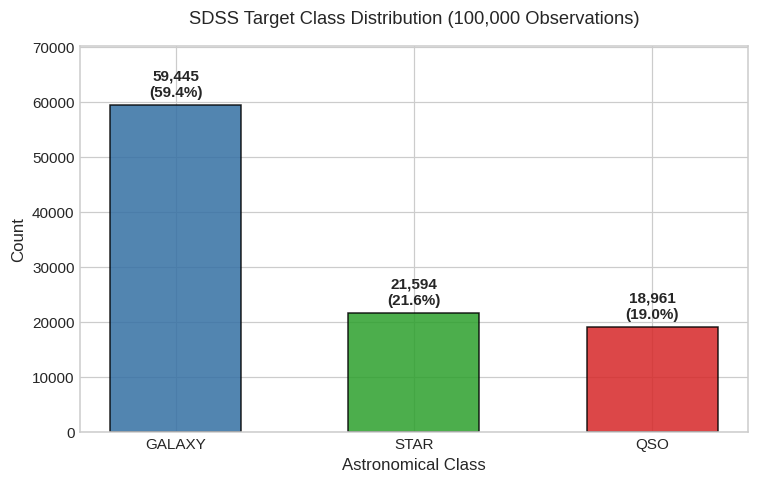
\includegraphics[width=0.52\textwidth]{figures/01_class_distribution.png}
    \caption{\textbf{Class distribution} across the 99,999 clean observations. Galaxies outnumber stars and quasars by nearly 3 to 1.}
    \label{fig:01_class_distribution}
\end{figure}

Because galaxies form a 60\% majority, a lazy model that guesses ``Galaxy'' every time would achieve 59.45\% accuracy while being totally useless for finding stars or quasars. For this reason, we rely on the \textbf{Macro-averaged F1-score}, which computes the harmonic mean of precision and recall for each class separately, and then averages them with equal weight:
\begin{equation}
    \text{Macro F1} = \frac{\text{F1}_{\text{GALAXY}} + \text{F1}_{\text{STAR}} + \text{F1}_{\text{QSO}}}{3}
\end{equation}

\subsection{Leakage-Free Train/Test Partitioning}
We split the 99,999 observations using a stratified 80/20 train/test split:
\begin{itemize}[noitemsep]
    \item \textbf{Training set:} 79,999 samples (59.45\% Galaxy, 21.59\% Star, 18.96\% Quasar).
    \item \textbf{Held-out test set:} 20,000 samples (59.44\% Galaxy, 21.60\% Star, 18.96\% Quasar).
\end{itemize}
To guarantee zero data leakage, a standard scaler (\texttt{StandardScaler}) was fitted \textbf{strictly on the training data}. The learned means and variances were then applied to normalize the test set.

% =========================================================================
% SECTION 2: PHASE 1 - BASELINE CLASSIFICATION
% =========================================================================
\section{Phase 1: Baseline Photometric Classification}

\subsection{The Core Idea: Raw Brightness Only}
In our first experiment, we test how well machine learning models can classify objects using only the raw brightness measured through five optical filters:
\begin{itemize}[noitemsep]
    \item $u$ (ultraviolet, ~355 nm), $g$ (green, ~468 nm), $r$ (red, ~616 nm), $i$ (near-infrared, ~748 nm), and $z$ (infrared, ~893 nm).
\end{itemize}
Here, we provide no engineered color ratios and no redshift information.

\subsection{Exploratory Data Analysis}
Figure~\ref{fig:01_eda_combined} shows the distribution of the five filter measurements and their correlation matrix. Figure~\ref{fig:01_boxplots} shows boxplots grouped by class.

\begin{figure}[H]
    \centering
    \begin{subfigure}[b]{0.48\textwidth}
        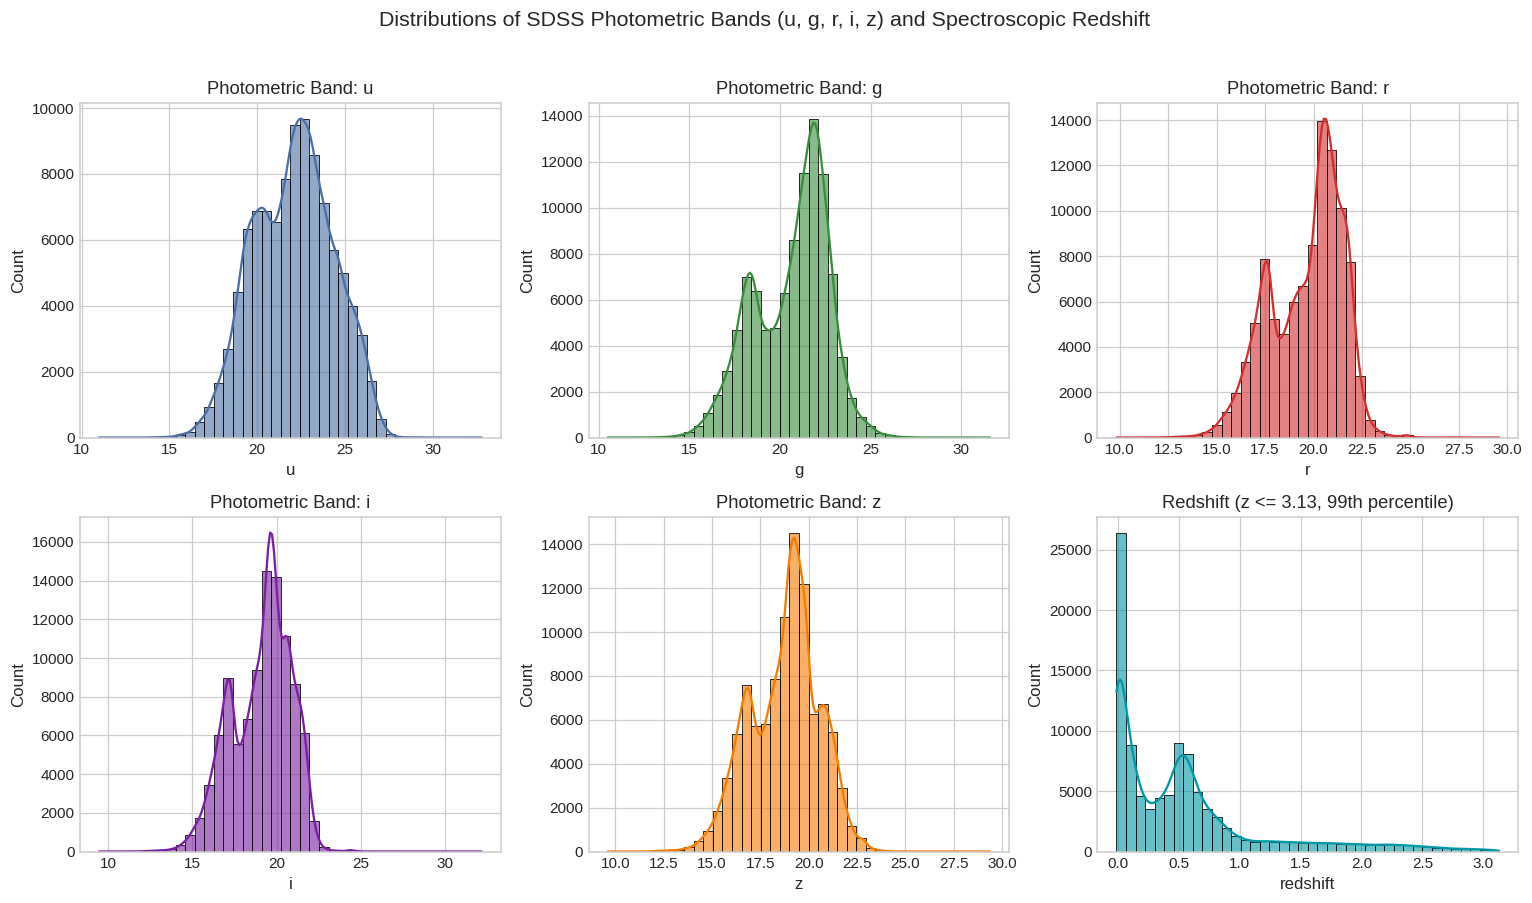
\includegraphics[width=\textwidth]{figures/01_photometric_and_redshift_distributions.png}
        \caption{Histograms of filters and redshift.}
        \label{fig:01_photo_dist}
    \end{subfigure}
    \hfill
    \begin{subfigure}[b]{0.48\textwidth}
        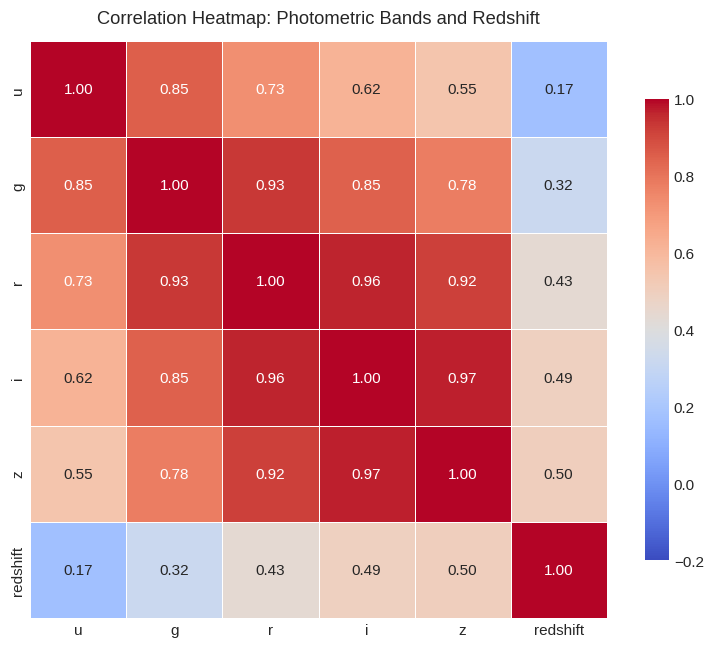
\includegraphics[width=\textwidth]{figures/01_correlation_heatmap.png}
        \caption{Inter-filter correlation heatmap.}
        \label{fig:01_corr_heatmap}
    \end{subfigure}
    \caption{\textbf{Exploratory analysis of raw features.} (a) Optical filters follow smooth bell-shaped curves. (b) Adjacent filters are highly collinear ($r = 0.94$ to $0.98$).}
    \label{fig:01_eda_combined}
\end{figure}

\begin{figure}[H]
    \centering
    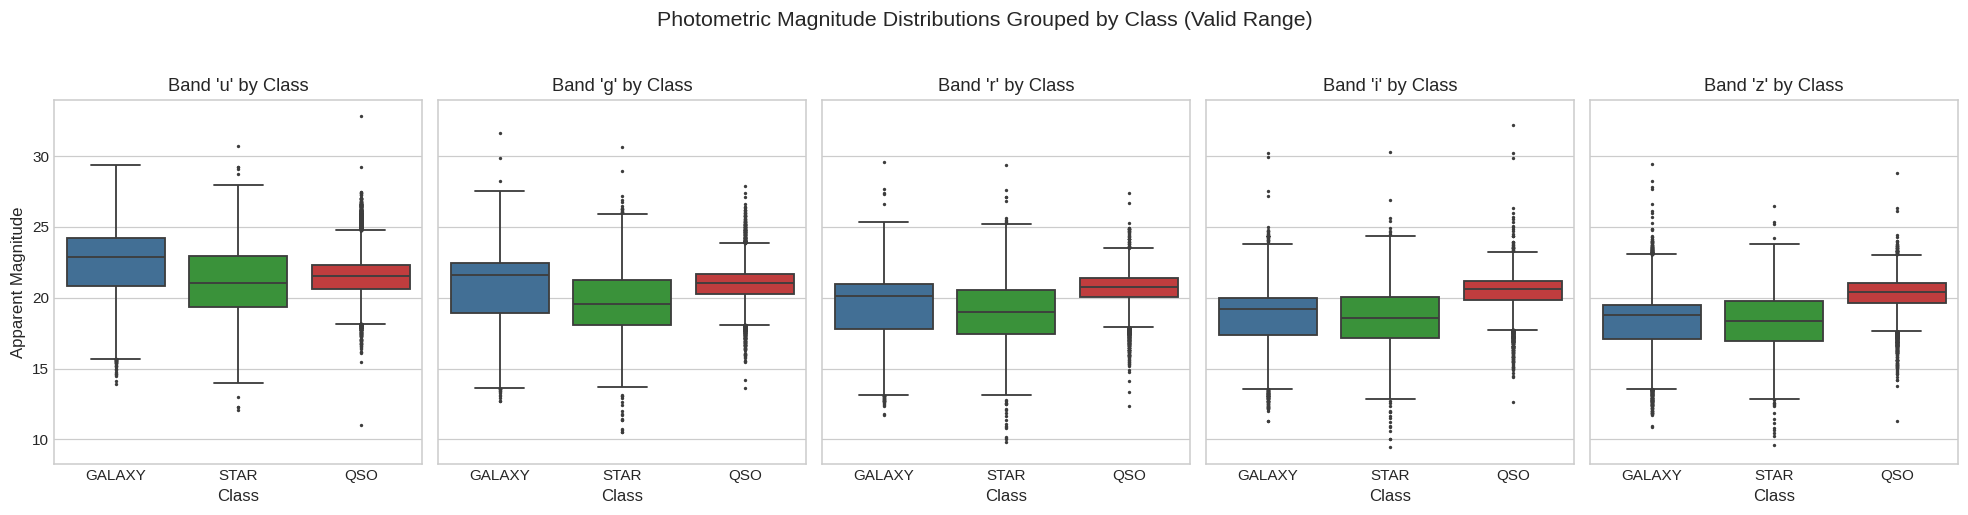
\includegraphics[width=0.72\textwidth]{figures/01_photometric_magnitude_boxplots.png}
    \caption{\textbf{Filter measurements grouped by class.} Stars (green) are brighter (lower magnitude) in red and infrared, but their brightness values overlap heavily with galaxies (blue) and quasars (red).}
    \label{fig:01_boxplots}
\end{figure}

\subsection{Evaluated Models and Numerical Results}
We trained four baseline classifiers on the identical 20,000 test observations:
\begin{enumerate}[noitemsep]
    \item \textbf{Logistic Regression:} Linear softmax model on standardized inputs.
    \item \textbf{K-Nearest Neighbors (KNN, $k=5$):} Distance-based neighborhood voting on standardized inputs.
    \item \textbf{Linear SVM (\texttt{LinearSVC}):} Margin-maximizing linear hyperplanes.
    \item \textbf{Random Forest (100 trees, depth 15):} Non-linear recursive partitioning on unscaled inputs.
\end{enumerate}

Table~\ref{tab:01_baseline_results} and Figure~\ref{fig:01_results_combined} present the measured performance.

\begin{table}[H]
\centering
\small
\caption{\textbf{Phase 1 Baseline Performance} on 20,000 test observations using raw 5-band photometry ($u, g, r, i, z$). Sorted by Macro F1-score.}
\label{tab:01_baseline_results}
\resizebox{\linewidth}{!}{
\begin{tabular}{lcccccccc}
\toprule
\textbf{Model} & \textbf{Accuracy} & \textbf{Macro F1} & \textbf{Macro Prec} & \textbf{Macro Rec} & \textbf{F1 (Gal)} & \textbf{F1 (Star)} & \textbf{F1 (QSO)} & \textbf{Train Time} \\
\midrule
\textbf{Random Forest} & \textbf{0.8656} & \textbf{0.8277} & 0.8429 & 0.8162 & \textbf{0.9192} & 0.7557 & \textbf{0.8083} & 33.84 s \\
\textbf{KNN ($k=5$)}    & 0.8625 & 0.8244 & 0.8345 & 0.8155 & 0.9180 & \textbf{0.7640} & 0.7912 & 0.37 s \\
\textbf{Logistic Reg.} & 0.7575 & 0.6702 & 0.7131 & 0.6743 & 0.8494 & 0.4351 & 0.7262 & 1.63 s \\
\textbf{Linear SVM}    & 0.7361 & 0.5974 & 0.7124 & 0.6336 & 0.8421 & 0.2327 & 0.7174 & 0.57 s \\
\bottomrule
\end{tabular}}
\end{table}

\begin{figure}[H]
    \centering
    \begin{subfigure}[b]{0.48\textwidth}
        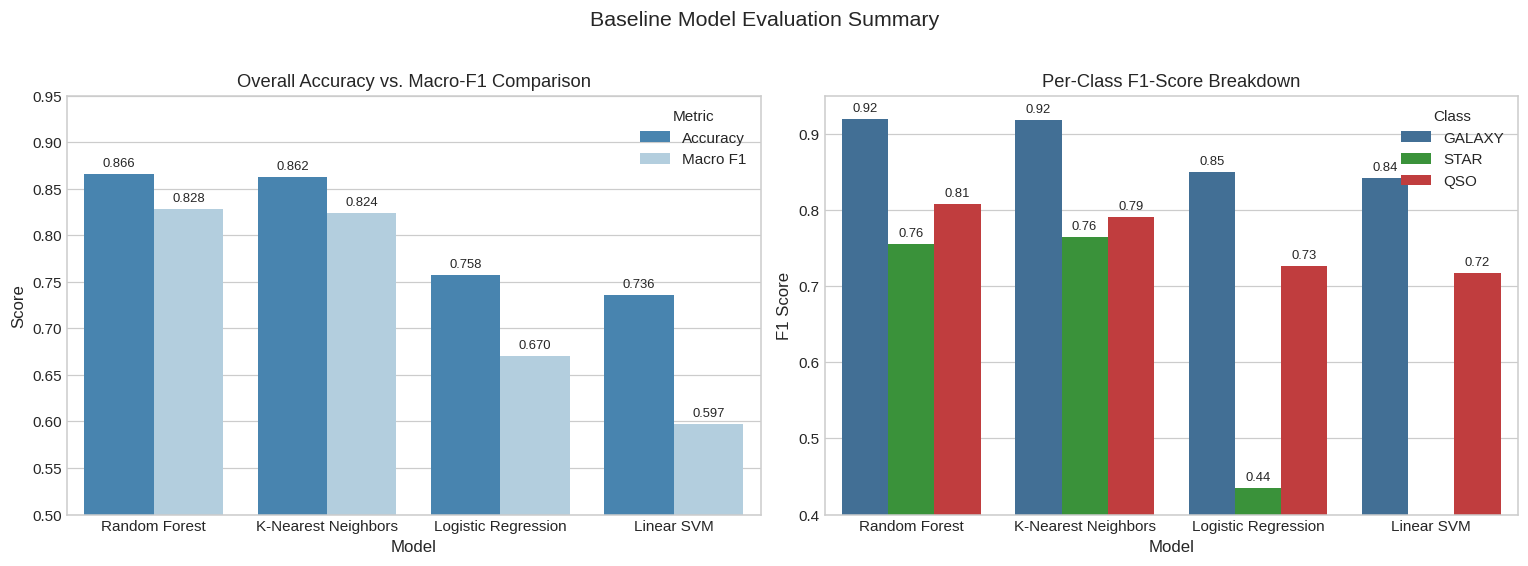
\includegraphics[width=\textwidth]{figures/01_baseline_model_comparison.png}
        \caption{Overall score and per-class breakdown.}
        \label{fig:01_comparison_bars}
    \end{subfigure}
    \hfill
    \begin{subfigure}[b]{0.48\textwidth}
        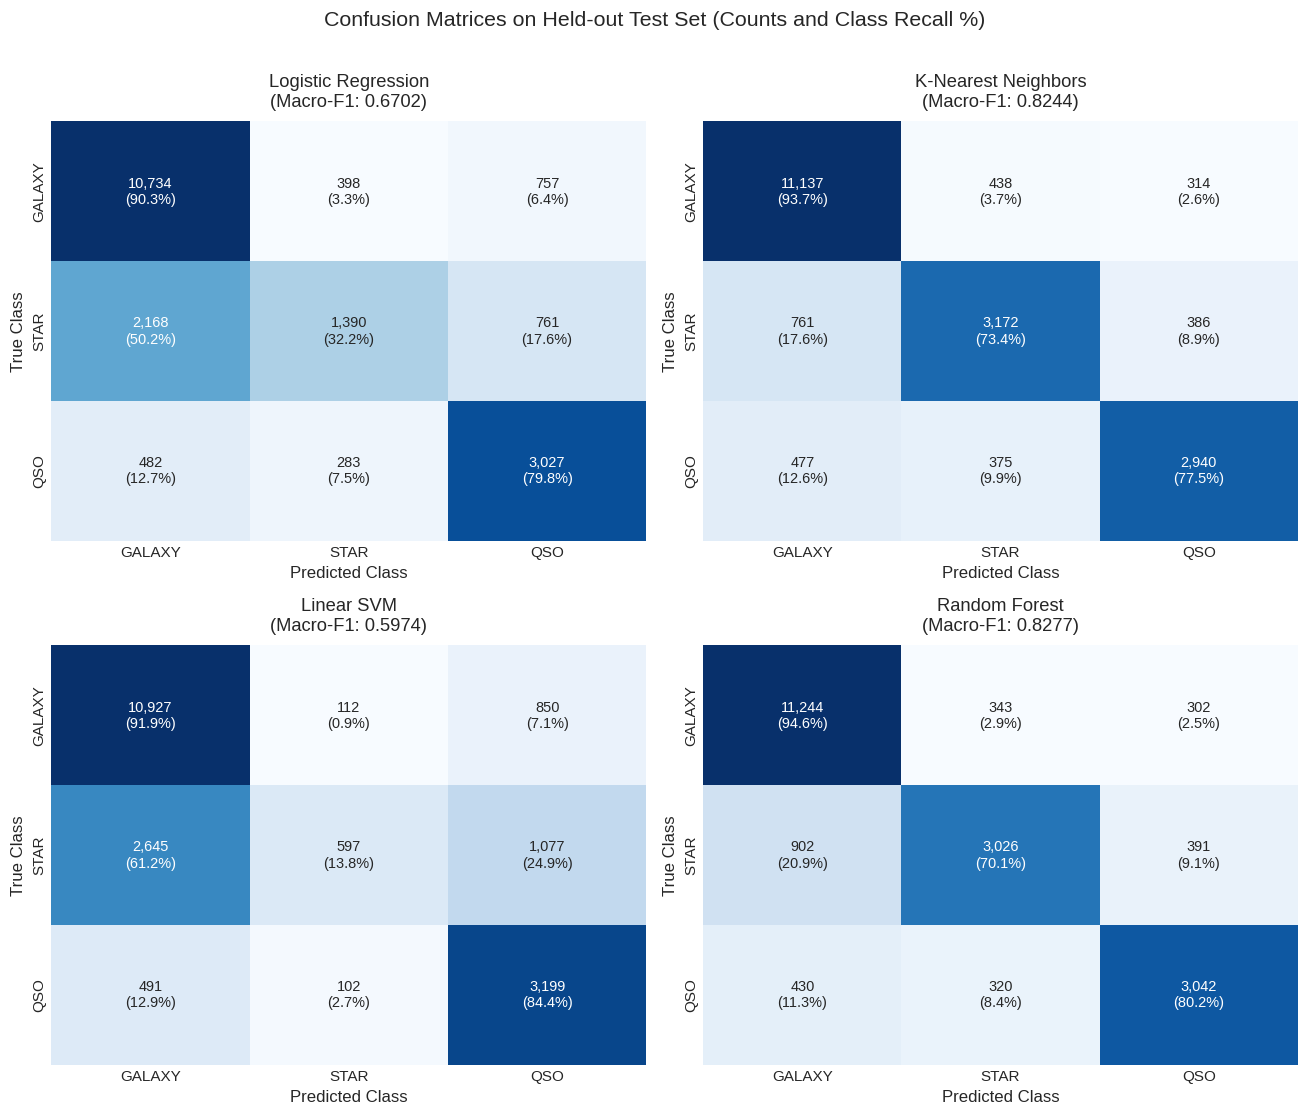
\includegraphics[width=\textwidth]{figures/01_baseline_confusion_matrices.png}
        \caption{Confusion matrices on 20,000 test samples.}
        \label{fig:01_confusion_matrices}
    \end{subfigure}
    \caption{\textbf{Baseline results.} (a) Non-linear models outperform linear models by 15--23 percentage points. (b) Linear SVM gets only 13.8\% recall on stars, incorrectly calling most stars ``Galaxies''.}
    \label{fig:01_results_combined}
\end{figure}

\subsection{Key Observations and Failure Modes}
\begin{enumerate}[noitemsep]
    \item \textbf{Non-Linear vs. Linear Divide:} Random Forest (0.8277 F1) and KNN (0.8244 F1) outperform Logistic Regression (0.6702 F1) and Linear SVM (0.5974 F1) by over 15 to 23 percentage points.
    \item \textbf{Why Linear Models Fail on Stars:} Figure~\ref{fig:01_confusion_matrices} reveals that Linear SVM catches only \textbf{597 out of 4,319 stars (13.82\% recall)}, misclassifying 2,395 stars as galaxies. A flat linear hyperplane cannot separate stars from galaxies in raw magnitude space without sweeping thousands of stars into the galaxy class.
    \item \textbf{The Distance Degeneracy:} Apparent brightness drops with distance ($F \propto 1/d^2$). A faint star nearby delivers the same amount of light to Earth as a brilliant quasar billions of light-years away. Raw brightness alone cannot separate them.
\end{enumerate}

% =========================================================================
% SECTION 3: PHASE 2 - COLOR FEATURE ENGINEERING
% =========================================================================
\section{Phase 2: Color Feature Engineering}

\subsection{The Core Idea: Scale-Free Color}
An object's \textbf{color} reveals its physical temperature and composition regardless of distance. A hot blue star looks blue whether it is close or far; a cool red star looks red. 

Because magnitudes follow Pogson's logarithmic scale ($m = -2.5 \log_{10}(F/F_0)$), subtracting two filter magnitudes calculates the logarithm of their flux ratio:
\begin{equation}
    m_1 - m_2 = -2.5 \log_{10}\left(\frac{F_1}{F_2}\right) = -2.5 \log_{10}\left(\frac{L_1 / 4\pi d^2}{L_2 / 4\pi d^2}\right) = -2.5 \log_{10}\left(\frac{L_1}{L_2}\right)
\end{equation}
The distance $d^2$ cancels out completely. The difference between two filters---called a \textbf{color index}---is a scale-free, distance-invariant measurement of true optical color.

\subsection{The Four Color Indices and Color-Color Diagrams}
We engineered four adjacent color features:
\begin{itemize}[noitemsep]
    \item \texttt{u\_g} $= u - g$: Measures ultraviolet excess. Active quasars shine with high UV energy, making \texttt{u\_g} low or negative.
    \item \texttt{g\_r} $= g - r$: Optical slope, separating hot blue stars from cool red stars.
    \item \texttt{r\_i} $= r - i$: Near-infrared slope, sensitive to cool stellar gas.
    \item \texttt{i\_z} $= i - z$: Deep infrared slope.
\end{itemize}

\begin{figure}[H]
    \centering
    \begin{subfigure}[b]{0.48\textwidth}
        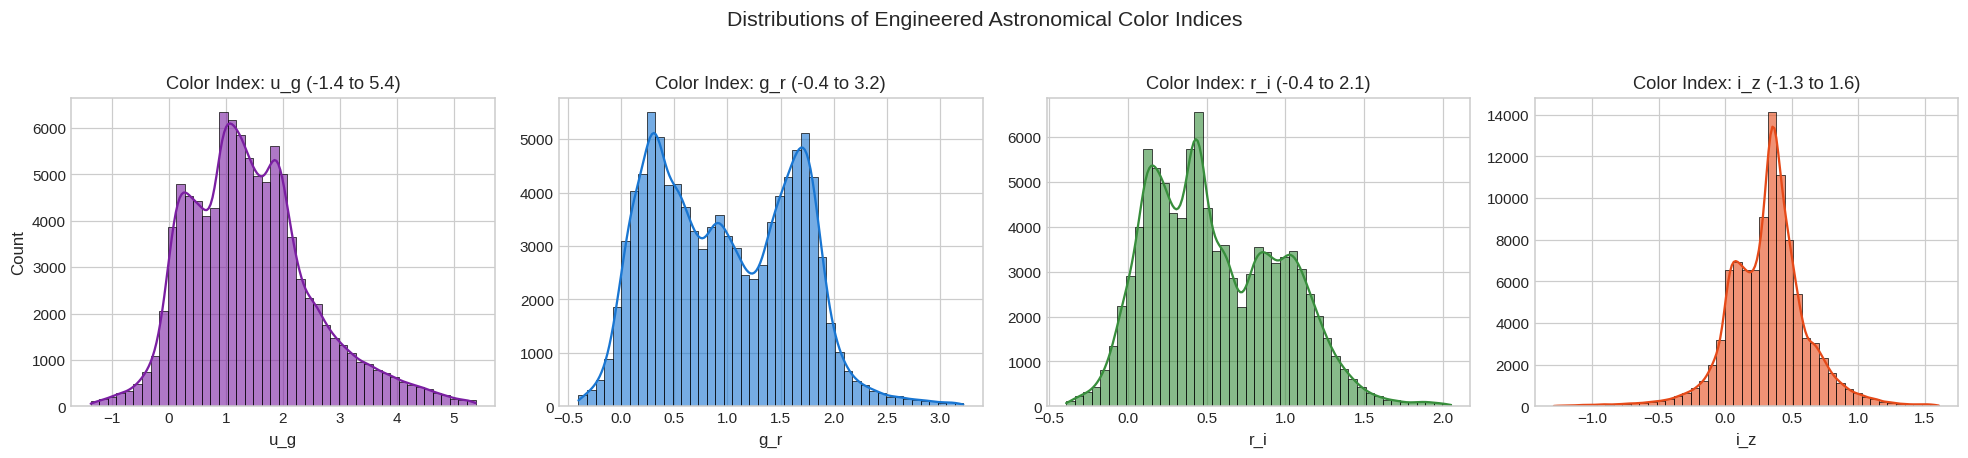
\includegraphics[width=\textwidth]{figures/02_color_index_distributions.png}
        \caption{Distributions of engineered colors.}
        \label{fig:02_color_dists}
    \end{subfigure}
    \hfill
    \begin{subfigure}[b]{0.48\textwidth}
        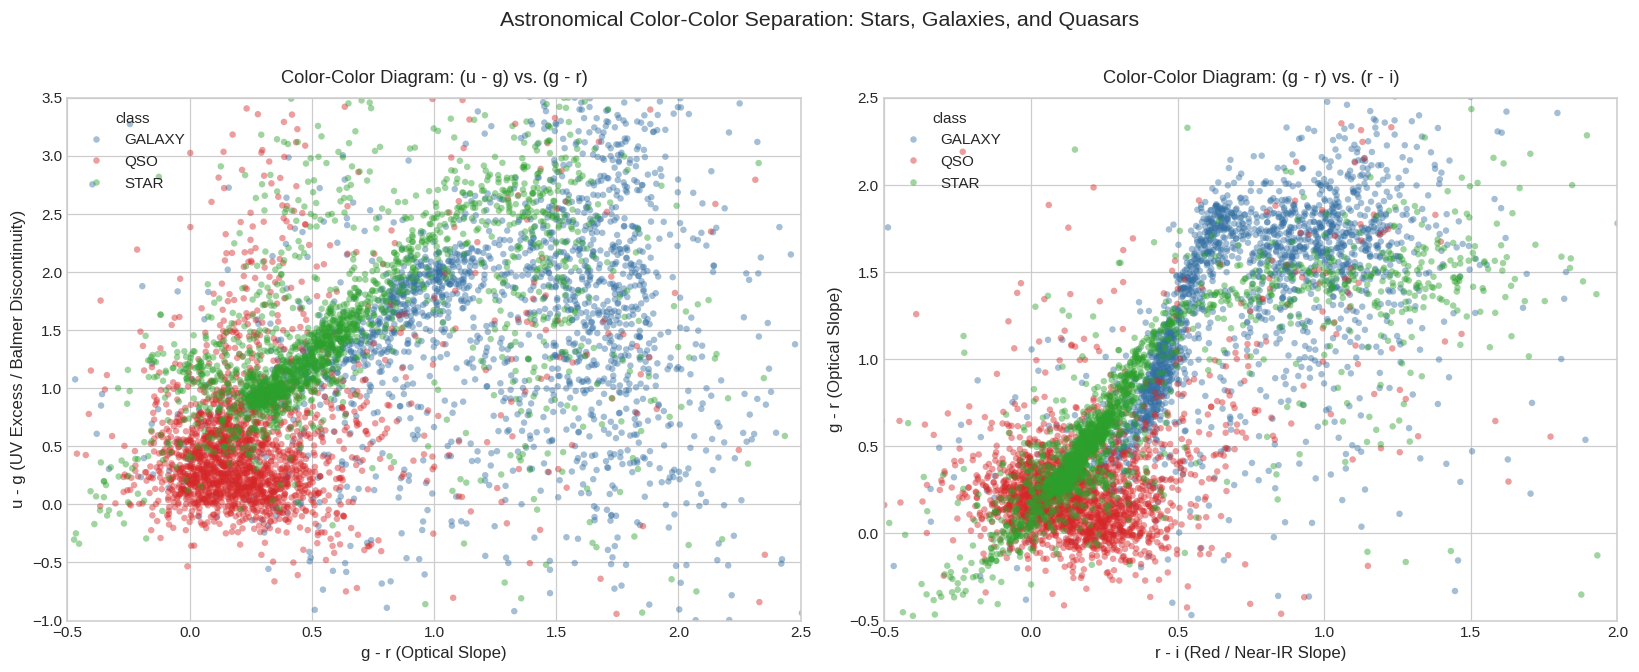
\includegraphics[width=\textwidth]{figures/02_color_color_diagrams.png}
        \caption{Astronomical color-color diagrams.}
        \label{fig:02_color_color}
    \end{subfigure}
    \caption{\textbf{Engineered color features.} (a) Color indices show clear bell curves. (b) Color-color plots reveal the \emph{stellar locus}: stars (green) form a narrow curve, while quasars (red) sit in the lower-left due to ultraviolet excess.}
    \label{fig:02_color_plots}
\end{figure}

\subsection{Experimental Results}
We compared the original 5 raw features against the expanded 9-feature set ($u, g, r, i, z$ plus the 4 colors). Table~\ref{tab:02_color_results} and Figure~\ref{fig:02_results_combined} report the results.

\begin{table}[H]
\centering
\small
\caption{\textbf{Phase 2 Comparison:} Original 5 features vs. 9 features (Original + Colors) on 20,000 test observations. Differences ($\Delta$) show percentage-point changes.}
\label{tab:02_color_results}
\resizebox{\linewidth}{!}{
\begin{tabular}{lccccccccccc}
\toprule
\textbf{Model} & \textbf{Acc (Orig)} & \textbf{Acc (Color)} & $\Delta$ \textbf{Acc} & \textbf{F1 (Orig)} & \textbf{F1 (Color)} & $\Delta$ \textbf{F1} & \textbf{F1 Star (Orig)} & \textbf{F1 Star (Color)} & $\Delta$ \textbf{F1 Star} & \textbf{F1 QSO (Color)} & \textbf{F1 Gal (Color)} \\
\midrule
\textbf{Random Forest} & 0.8656 & \textbf{0.8847} & \textbf{+1.91\%} & 0.8277 & \textbf{0.8514} & \textbf{+2.36\%} & 0.7557 & \textbf{0.8062} & \textbf{+5.05\%} & 0.8151 & \textbf{0.9329} \\
\textbf{KNN ($k=5$)}    & 0.8625 & \textbf{0.8761} & \textbf{+1.36\%} & 0.8244 & \textbf{0.8415} & \textbf{+1.72\%} & 0.7640 & \textbf{0.7960} & \textbf{+3.20\%} & 0.8023 & 0.9263 \\
\textbf{Logistic Reg.} & 0.7575 & 0.7577 & +0.01\% & 0.6702 & 0.6704 & +0.02\% & 0.4351 & 0.4354 & +0.04\% & 0.7262 & 0.8495 \\
\textbf{Linear SVM}    & 0.7361 & 0.7361 & +0.00\% & 0.5974 & 0.5974 & +0.00\% & 0.2327 & 0.2327 & +0.00\% & 0.7174 & 0.8421 \\
\bottomrule
\end{tabular}}
\end{table}

\begin{figure}[H]
    \centering
    \begin{subfigure}[b]{0.48\textwidth}
        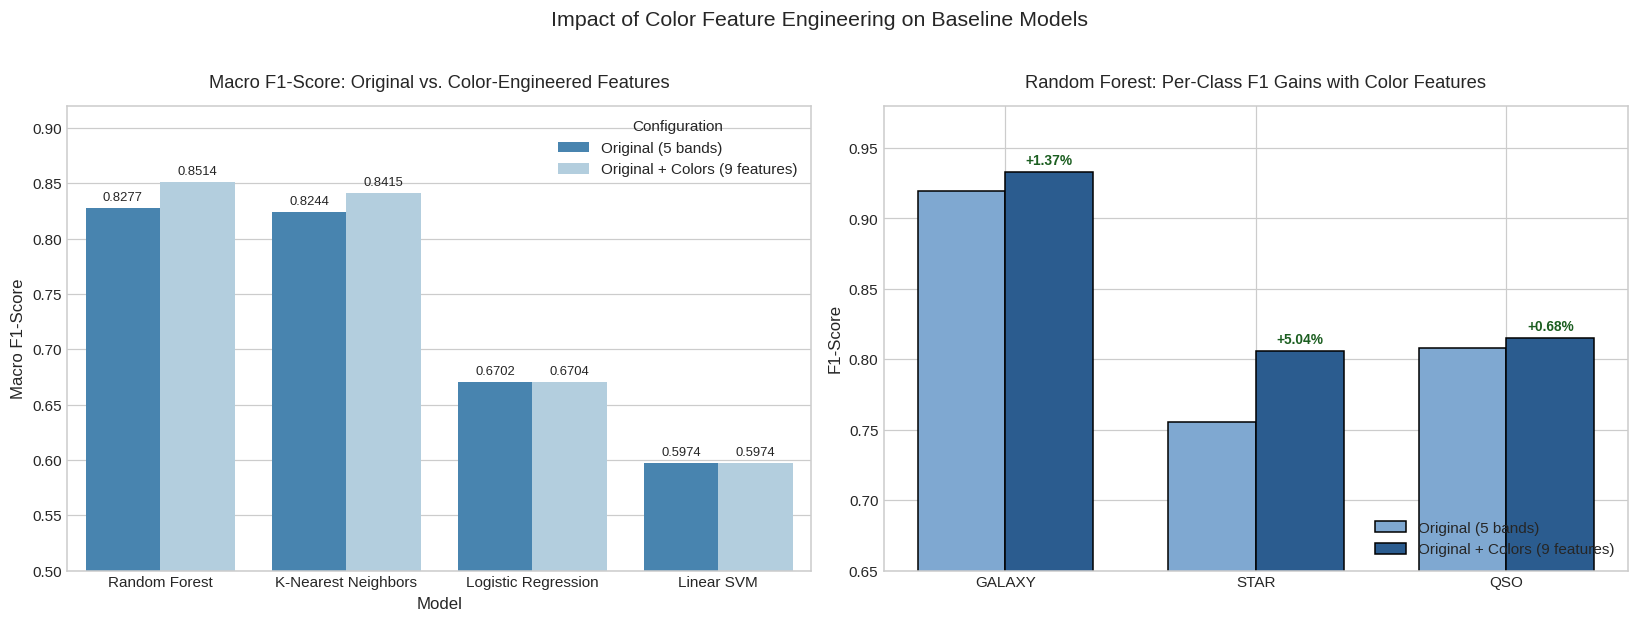
\includegraphics[width=\textwidth]{figures/02_color_engineering_performance_comparison.png}
        \caption{Performance gains by model and class.}
        \label{fig:02_gains}
    \end{subfigure}
    \hfill
    \begin{subfigure}[b]{0.48\textwidth}
        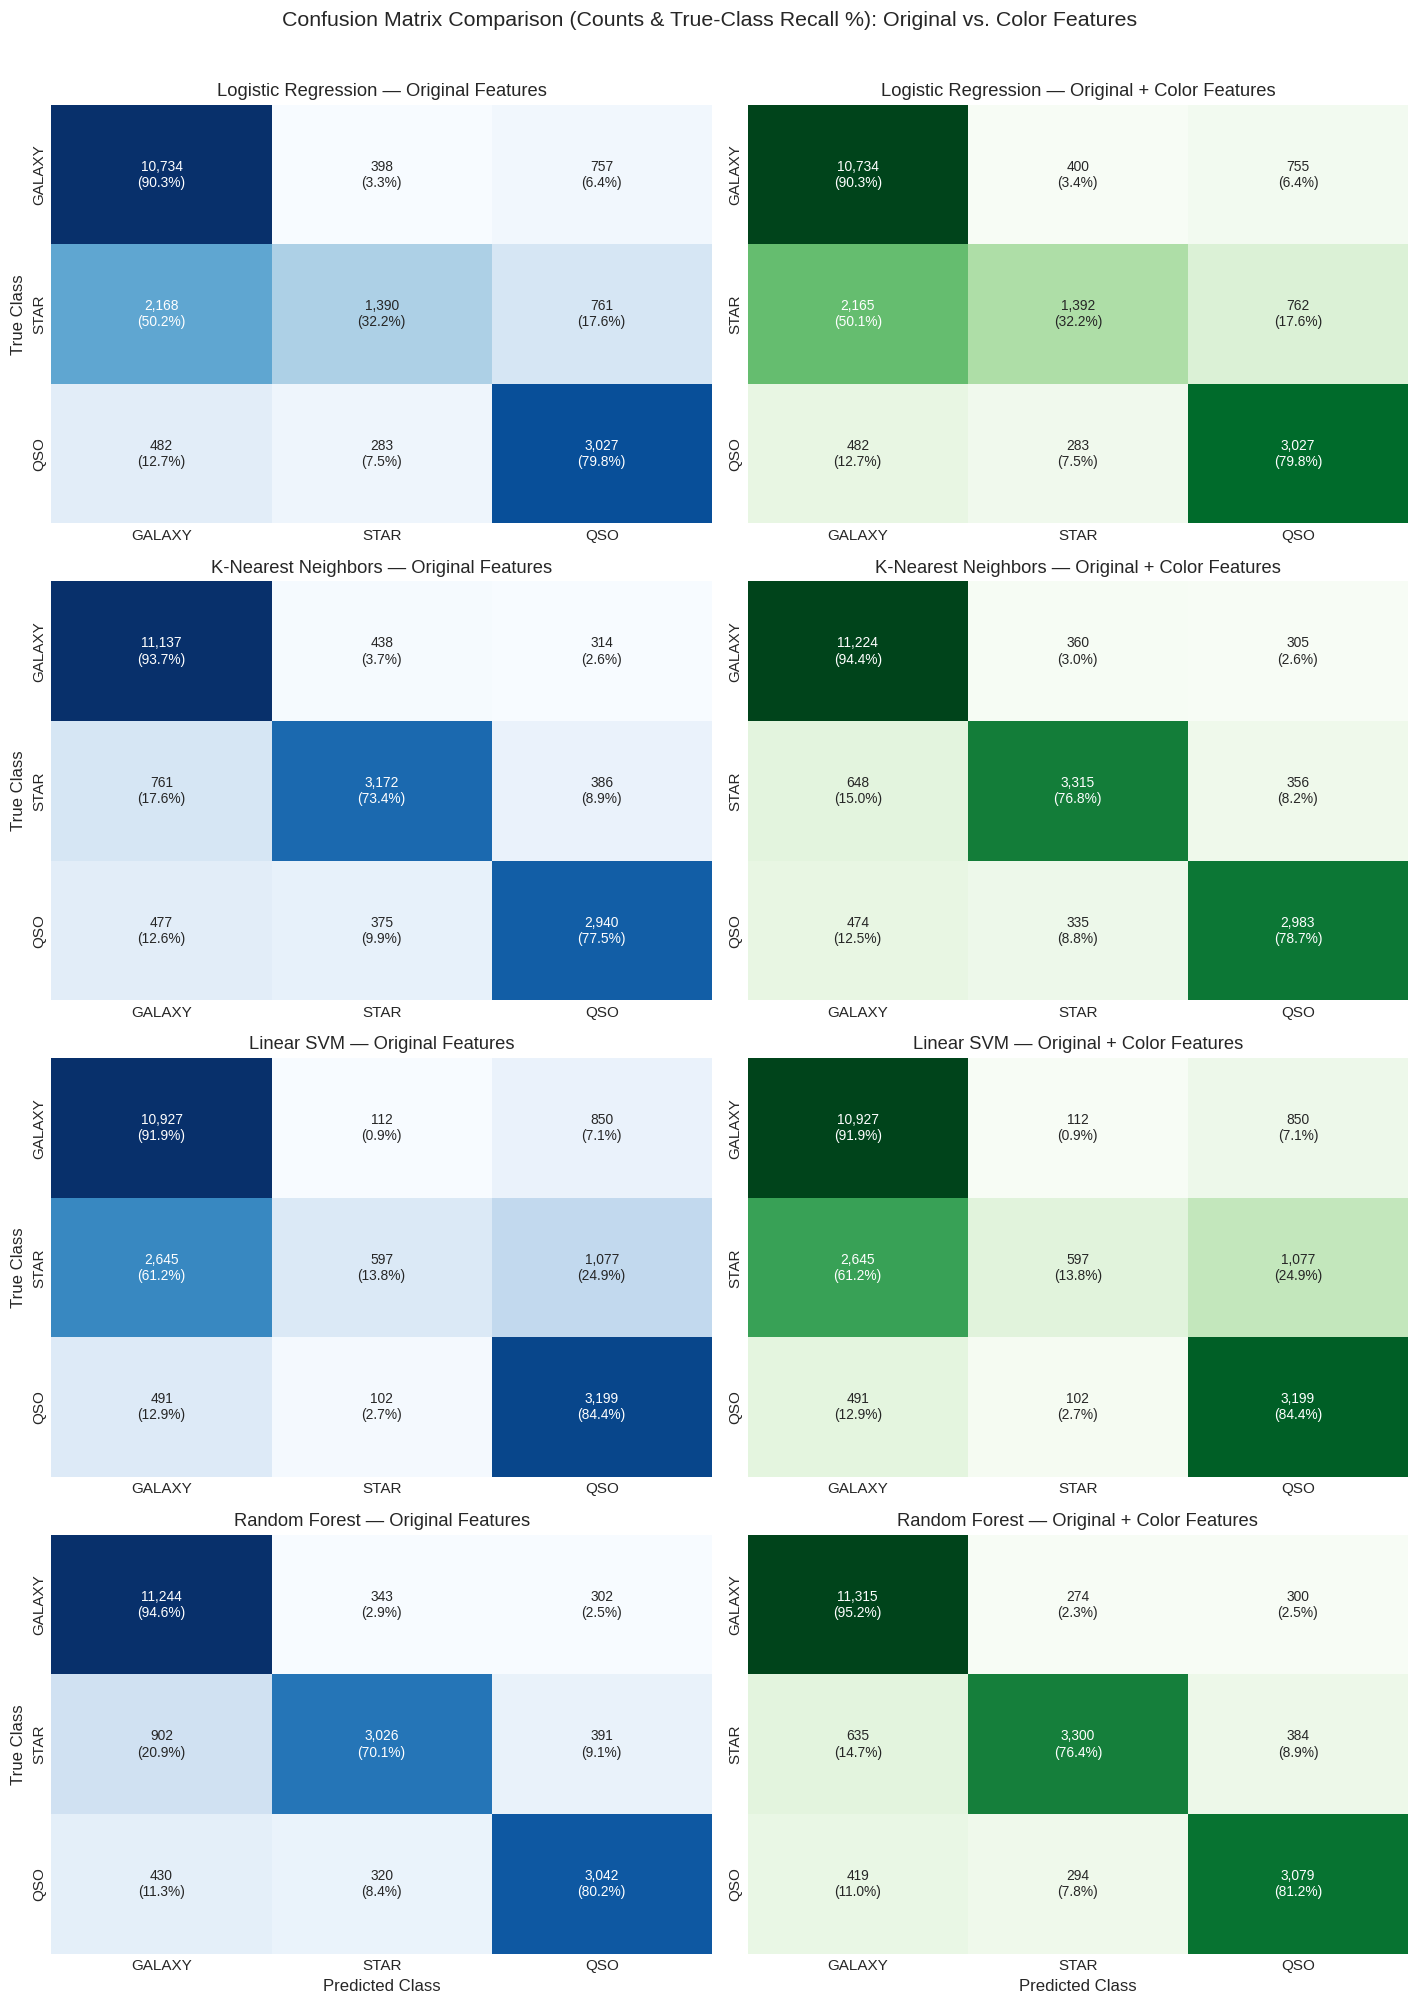
\includegraphics[width=\textwidth]{figures/02_color_engineering_confusion_matrices.png}
        \caption{Confusion matrix comparison.}
        \label{fig:02_cm_compare}
    \end{subfigure}
    \caption{\textbf{Impact of color features.} (a) Stars gain +5.05 percentage points in Random Forest. (b) Random Forest cuts mistakes by 382.}
    \label{fig:02_results_combined}
\end{figure}

\subsection{Observations: Why Models Diverged}
\begin{enumerate}[noitemsep]
    \item \textbf{Random Forest Cuts 382 Mistakes:} Accuracy rose to \textbf{88.47\%} (+1.91 pp) and Macro F1 rose to \textbf{0.8514} (+2.36 pp), reducing test errors from 2,688 down to 2,306 (a \textbf{14.2\% relative error reduction}).
    \item \textbf{Stars Were the Big Winner:} Stellar F1 in Random Forest leaped by \textbf{+5.05 percentage points} (0.7557 to 0.8062). As seen in Figure~\ref{fig:02_color_color}, stars follow a narrow, curved track in color-color space. Color indices allow tree models to isolate stars cleanly.
    \item \textbf{Why Linear Classifiers Saw 0.00\% Gain:} Linear SVM showed exactly 0.00\% change, and Logistic Regression moved by +0.02\%. Color indices are linear subtractions ($u - g$). The 9-dimensional space spans the exact same 5-dimensional linear subspace ($\text{rank} = 5$). Any flat hyperplane in 9D can already be drawn in 5D. Linear models cannot extract curved interactions without non-linear kernels.
    \item \textbf{Why Decision Trees Benefited:} Decision trees make axis-aligned cuts ($x \le \theta$). Separating a diagonal relationship ($u - g \le \theta$) using only $u$ and $g$ requires a clumsy staircase of dozens of splits. Giving the tree $u - g$ directly allows a single, clean cut at depth 1.
\end{enumerate}

% =========================================================================
% SECTION 4: PHASE 3 - REDSHIFT ABLATION STUDY
% =========================================================================
\section{Phase 3: Redshift Ablation Study}

\subsection{The Core Idea: What is an Ablation Study?}
An \textbf{ablation study} systematically removes or adds a component to measure its exact marginal value. Here, we ask: \emph{How much does spectroscopic redshift ($z$) improve classification accuracy, and how does its value compare to color features?}

\subsection{The Physics of Redshift}
Redshift measures how much spectral lines are stretched to redder wavelengths:
\begin{equation}
    z = \frac{\lambda_{\text{observed}} - \lambda_{\text{rest}}}{\lambda_{\text{rest}}}
\end{equation}
The three classes naturally separate in redshift (Figure~\ref{fig:03_redshift_chars}):
\begin{itemize}[noitemsep]
    \item \textbf{Stars ($z \approx 0$):} Inside the Milky Way, speeds rarely exceed 500 km/s. Stellar redshifts cluster tightly near zero (mean $z = -0.0001$). In fact, \textbf{63.36\% of stars have negative redshifts (blueshifts)} because their orbit carries them toward the Sun!
    \item \textbf{Galaxies ($0.01 \le z \le 1.5$):} Moderate cosmological distances (median $z = 0.46$).
    \item \textbf{Quasars ($z \ge 0.5$ up to $7.0$):} Distant active galactic nuclei (median $z = 1.62$). Every single quasar in the dataset has a positive redshift.
\end{itemize}

\begin{figure}[H]
    \centering
    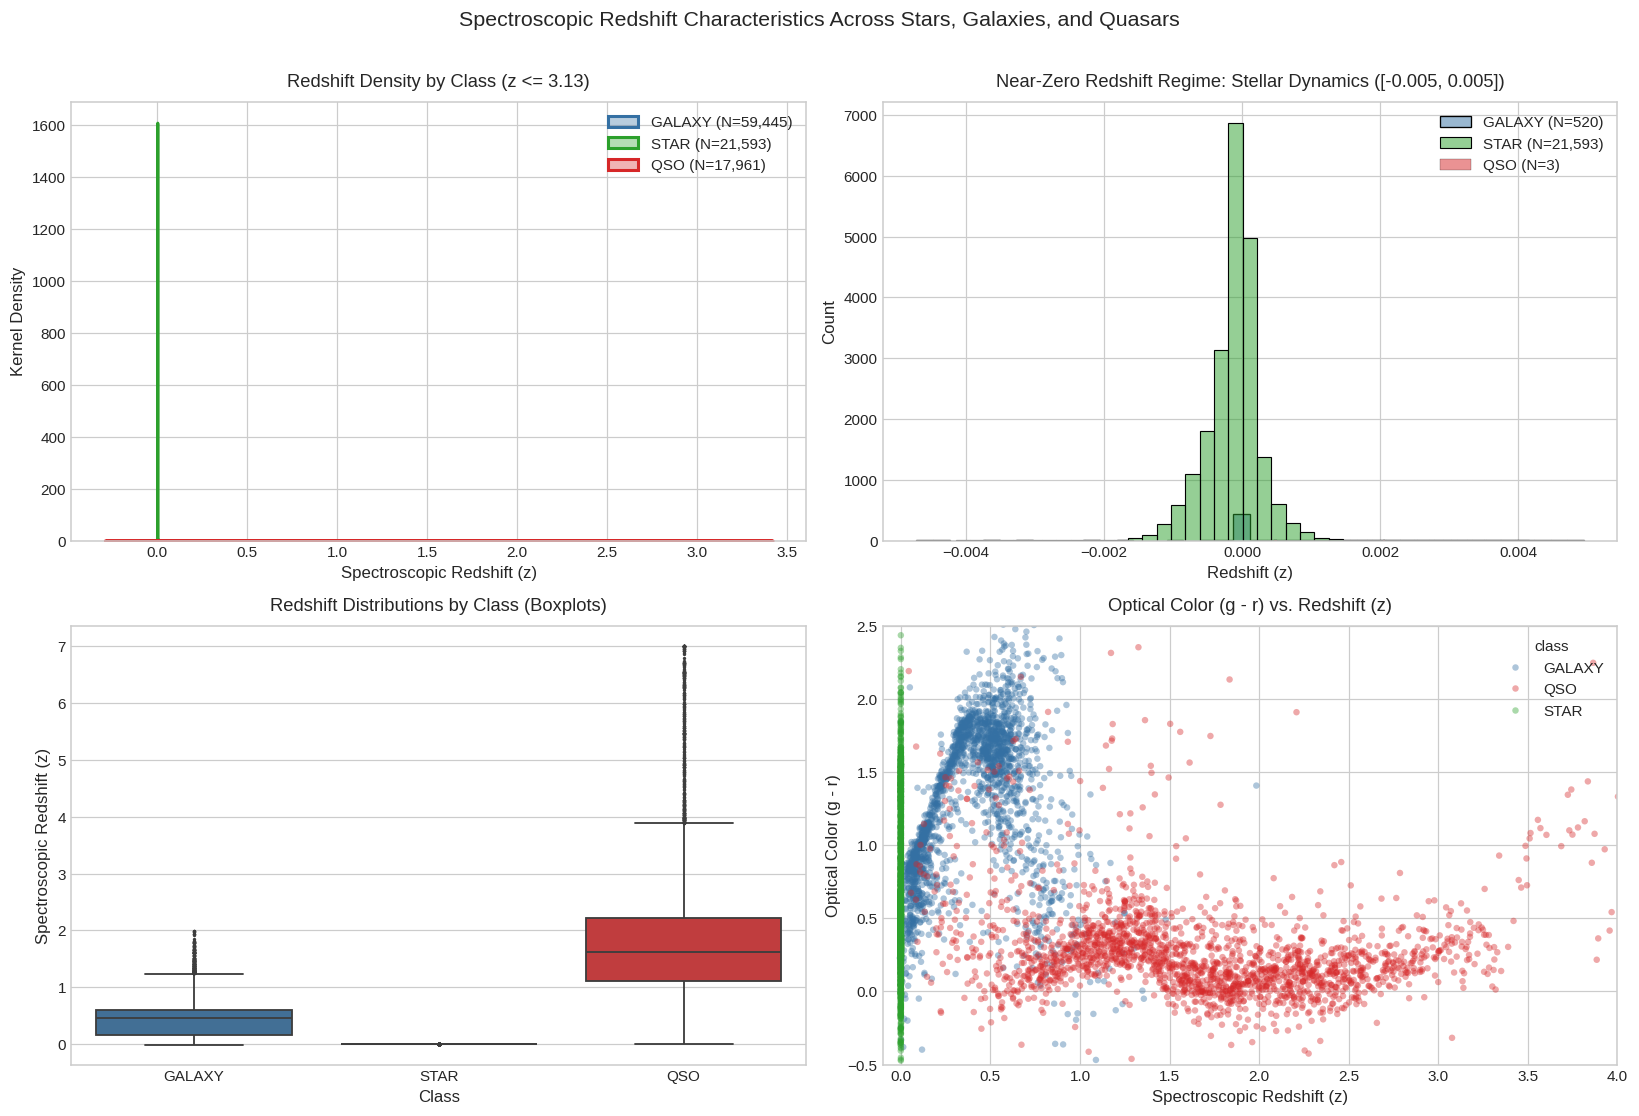
\includegraphics[width=0.72\textwidth]{figures/03_redshift_characteristics_by_class.png}
    \caption{\textbf{Redshift characteristics across classes.} (a) Density plot showing natural class separation. (b) Zoom on stars near $z = 0$, where 63.4\% have blueshifts. (c) Boxplots showing quasars reaching past $z = 6$. (d) Color vs. redshift showing clear grouping.}
    \label{fig:03_redshift_chars}
\end{figure}

\subsection{Experimental Results Across Three Configurations}
We evaluated three progressive configurations:
\begin{enumerate}[noitemsep]
    \item \textbf{Configuration 1 (Photometry only):} 5 raw bands ($u, g, r, i, z$).
    \item \textbf{Configuration 2 (Photometry + Redshift):} 6 features ($u, g, r, i, z, \text{redshift}$).
    \item \textbf{Configuration 3 (Photometry + Colors + Redshift):} 10 features ($u, g, r, i, z, u-g, g-r, r-i, i-z, \text{redshift}$).
\end{enumerate}

Table~\ref{tab:03_ablation_results} and Figure~\ref{fig:03_results_combined} present the results.

\begin{table}[H]
\centering
\small
\caption{\textbf{Phase 3 Redshift Ablation Results} on 20,000 test observations. Differences ($\Delta$) show percentage-point gains when adding redshift to raw photometry.}
\label{tab:03_ablation_results}
\resizebox{\linewidth}{!}{
\begin{tabular}{lcccccccccc}
\toprule
\textbf{Model} & \textbf{Acc (Cfg 1)} & \textbf{Acc (Cfg 2)} & \textbf{Acc (Cfg 3)} & $\Delta$ \textbf{Acc (z)} & \textbf{F1 (Cfg 1)} & \textbf{F1 (Cfg 2)} & \textbf{F1 (Cfg 3)} & $\Delta$ \textbf{F1 (z)} & \textbf{F1 Star (Cfg 3)} & \textbf{F1 QSO (Cfg 3)} \\
\midrule
\textbf{Random Forest} & 0.8656 & 0.9797 & \textbf{0.9800} & \textbf{+11.40\%} & 0.8277 & 0.9762 & \textbf{0.9767} & \textbf{+14.84\%} & \textbf{0.9976} & \textbf{0.9492} \\
\textbf{KNN ($k=5$)}    & 0.8625 & \textbf{0.9637} & 0.9558 & \textbf{+10.12\%} & 0.8244 & \textbf{0.9594} & 0.9507 & \textbf{+13.50\%} & 0.9474 & 0.9414 \\
\textbf{Logistic Reg.} & 0.7575 & \textbf{0.9578} & 0.9577 & \textbf{+20.03\%} & 0.6702 & \textbf{0.9515} & 0.9515 & \textbf{+28.13\%} & 0.9733 & 0.9164 \\
\textbf{Linear SVM}    & 0.7361 & \textbf{0.9386} & 0.9386 & \textbf{+20.25\%} & 0.5974 & \textbf{0.9315} & 0.9315 & \textbf{+33.40\%} & 0.9375 & 0.9082 \\
\bottomrule
\end{tabular}}
\end{table}

\begin{figure}[H]
    \centering
    \begin{subfigure}[b]{0.48\textwidth}
        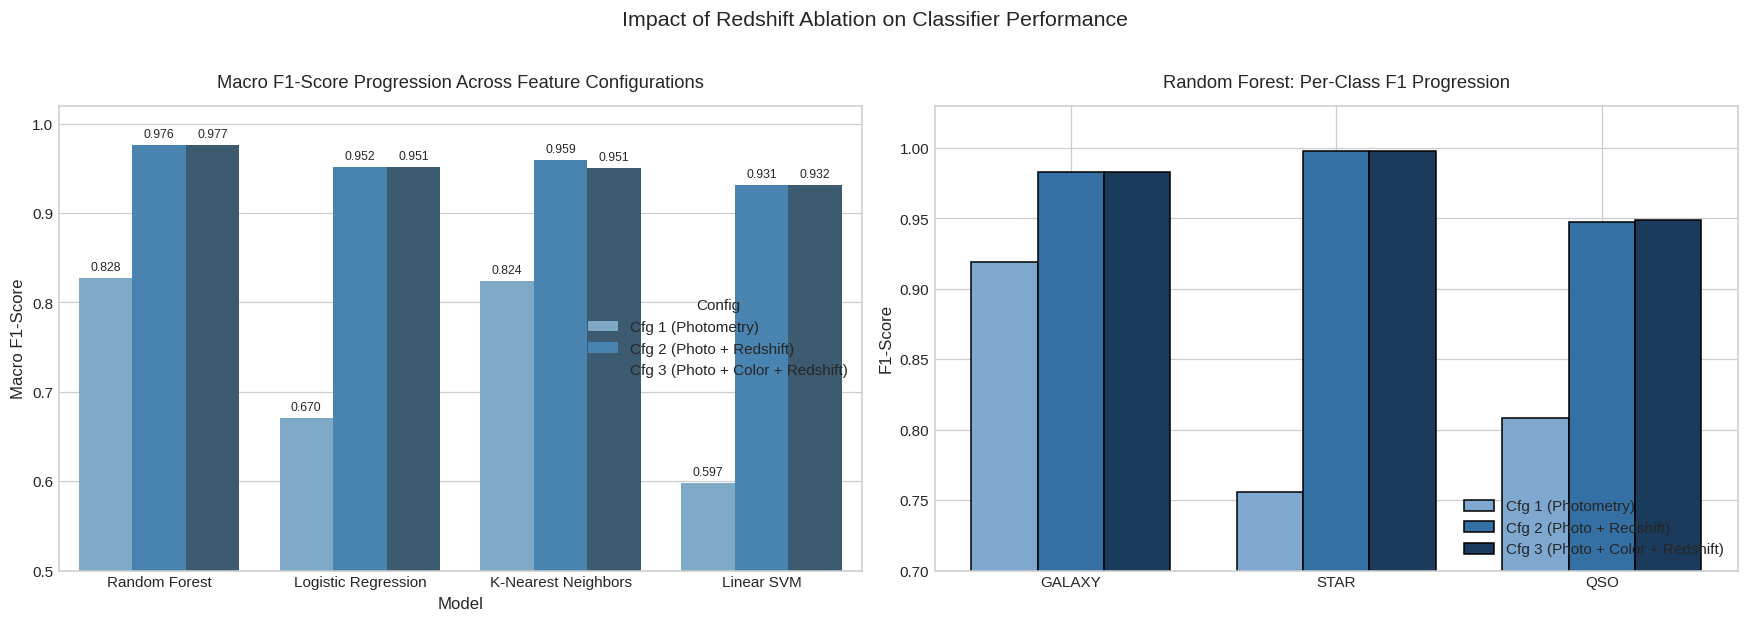
\includegraphics[width=\textwidth]{figures/03_redshift_ablation_performance_comparison.png}
        \caption{Performance jumps across configurations.}
        \label{fig:03_ablation_bars}
    \end{subfigure}
    \hfill
    \begin{subfigure}[b]{0.48\textwidth}
        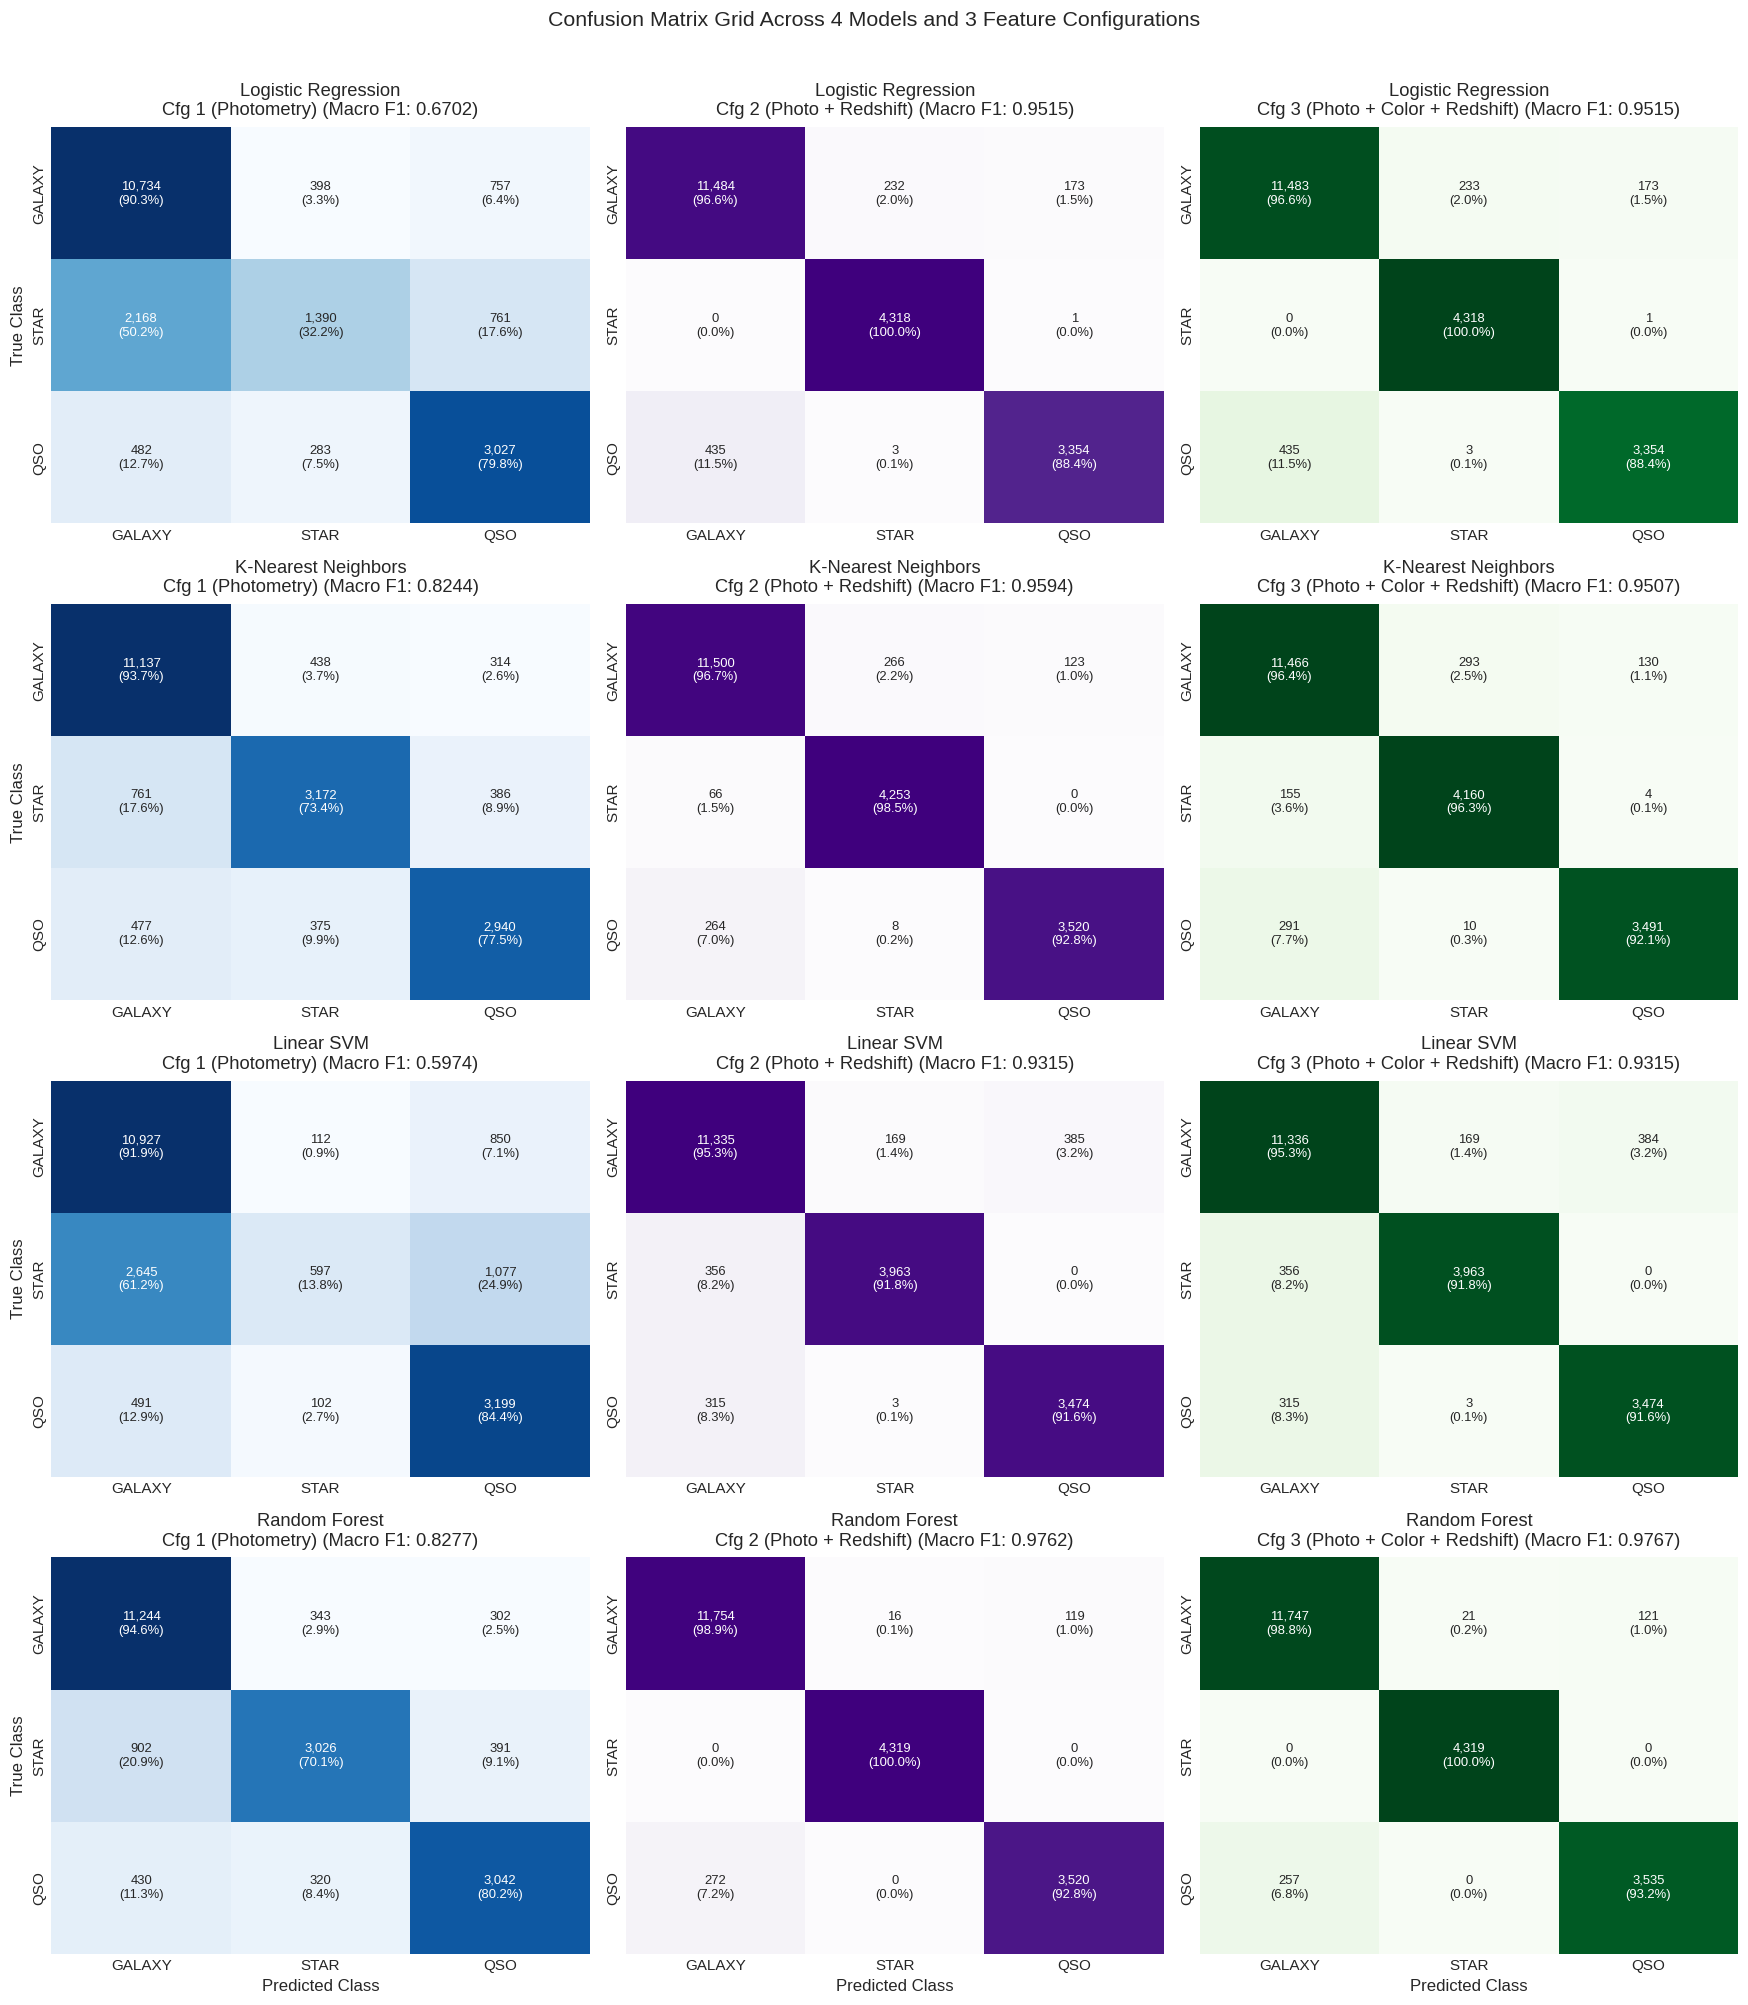
\includegraphics[width=\textwidth]{figures/03_redshift_ablation_confusion_matrices.png}
        \caption{Grid of confusion matrices.}
        \label{fig:03_ablation_cm}
    \end{subfigure}
    \caption{\textbf{Impact of redshift.} (a) Adding redshift causes a huge vertical jump across all models. (b) Random Forest mistakes drop from 2,688 down to just 399.}
    \label{fig:03_results_combined}
\end{figure}

\subsection{Observations: Redshift Dominates Completely}
\begin{enumerate}[noitemsep]
    \item \textbf{85.2\% Error Drop in Random Forest:} Test mistakes plummeted from \textbf{2,688 to 399 errors}, reaching \textbf{98.00\% Accuracy} and \textbf{0.9767 Macro F1}.
    \item \textbf{Near-Perfect Stellar Identification:} Stellar F1 reached \textbf{0.9976} with \textbf{100.0\% recall} (all 4,319 test stars correctly identified). Redshift acts as an absolute veto against confusing stars with distant quasars.
    \item \textbf{Linear Models Rescued:} Linear SVM leaped by \textbf{+33.40 pp} (0.5974 to 0.9315 F1), and Logistic Regression gained \textbf{+28.13 pp}. Redshift provides a straight, near-linearly separable axis separating local stars from distant quasars.
    \item \textbf{Redshift vs. Color Disentanglement:} Adding color on top of redshift (Cfg 2 vs. Cfg 3) improved Random Forest by only +0.05 pp and slightly hurt KNN (-0.87 pp) because redundant features diluted the Euclidean distance metric. Redshift carries the primary physical signal.
    \item \textbf{The Practical Catch:} Redshift delivers ~98\% accuracy, but \textbf{spectroscopic redshift is expensive}. Spectroscopy takes hours of telescope time per object, whereas cameras photograph millions in seconds. Therefore, while Phase 3 establishes the theoretical maximum ceiling, \textbf{Phase 2 (Color Engineering) remains the true operational model for real-time sky surveys}.
\end{enumerate}

% =========================================================================
% SECTION 5: PHASE 4 - FEATURE SELECTION
% =========================================================================
\section{Phase 4: Feature Selection and Importance Analysis}

\subsection{The Core Idea: Building Leaner Models}
Can we build a model that matches our 98\% accuracy ceiling while using far fewer features? Smaller models train faster, run with lower latency, and require less data transfer.

\subsection{Feature Importance: MDI vs. Permutation}
We evaluated feature importance using two methods:
\begin{itemize}[noitemsep]
    \item \textbf{Mean Decrease in Impurity (MDI / Gini):} Counts how much impurity decision tree splits remove during training.
    \item \textbf{Permutation Importance:} Measures the drop in test-set Macro F1 when a feature is randomly shuffled.
\end{itemize}

\begin{figure}[H]
    \centering
    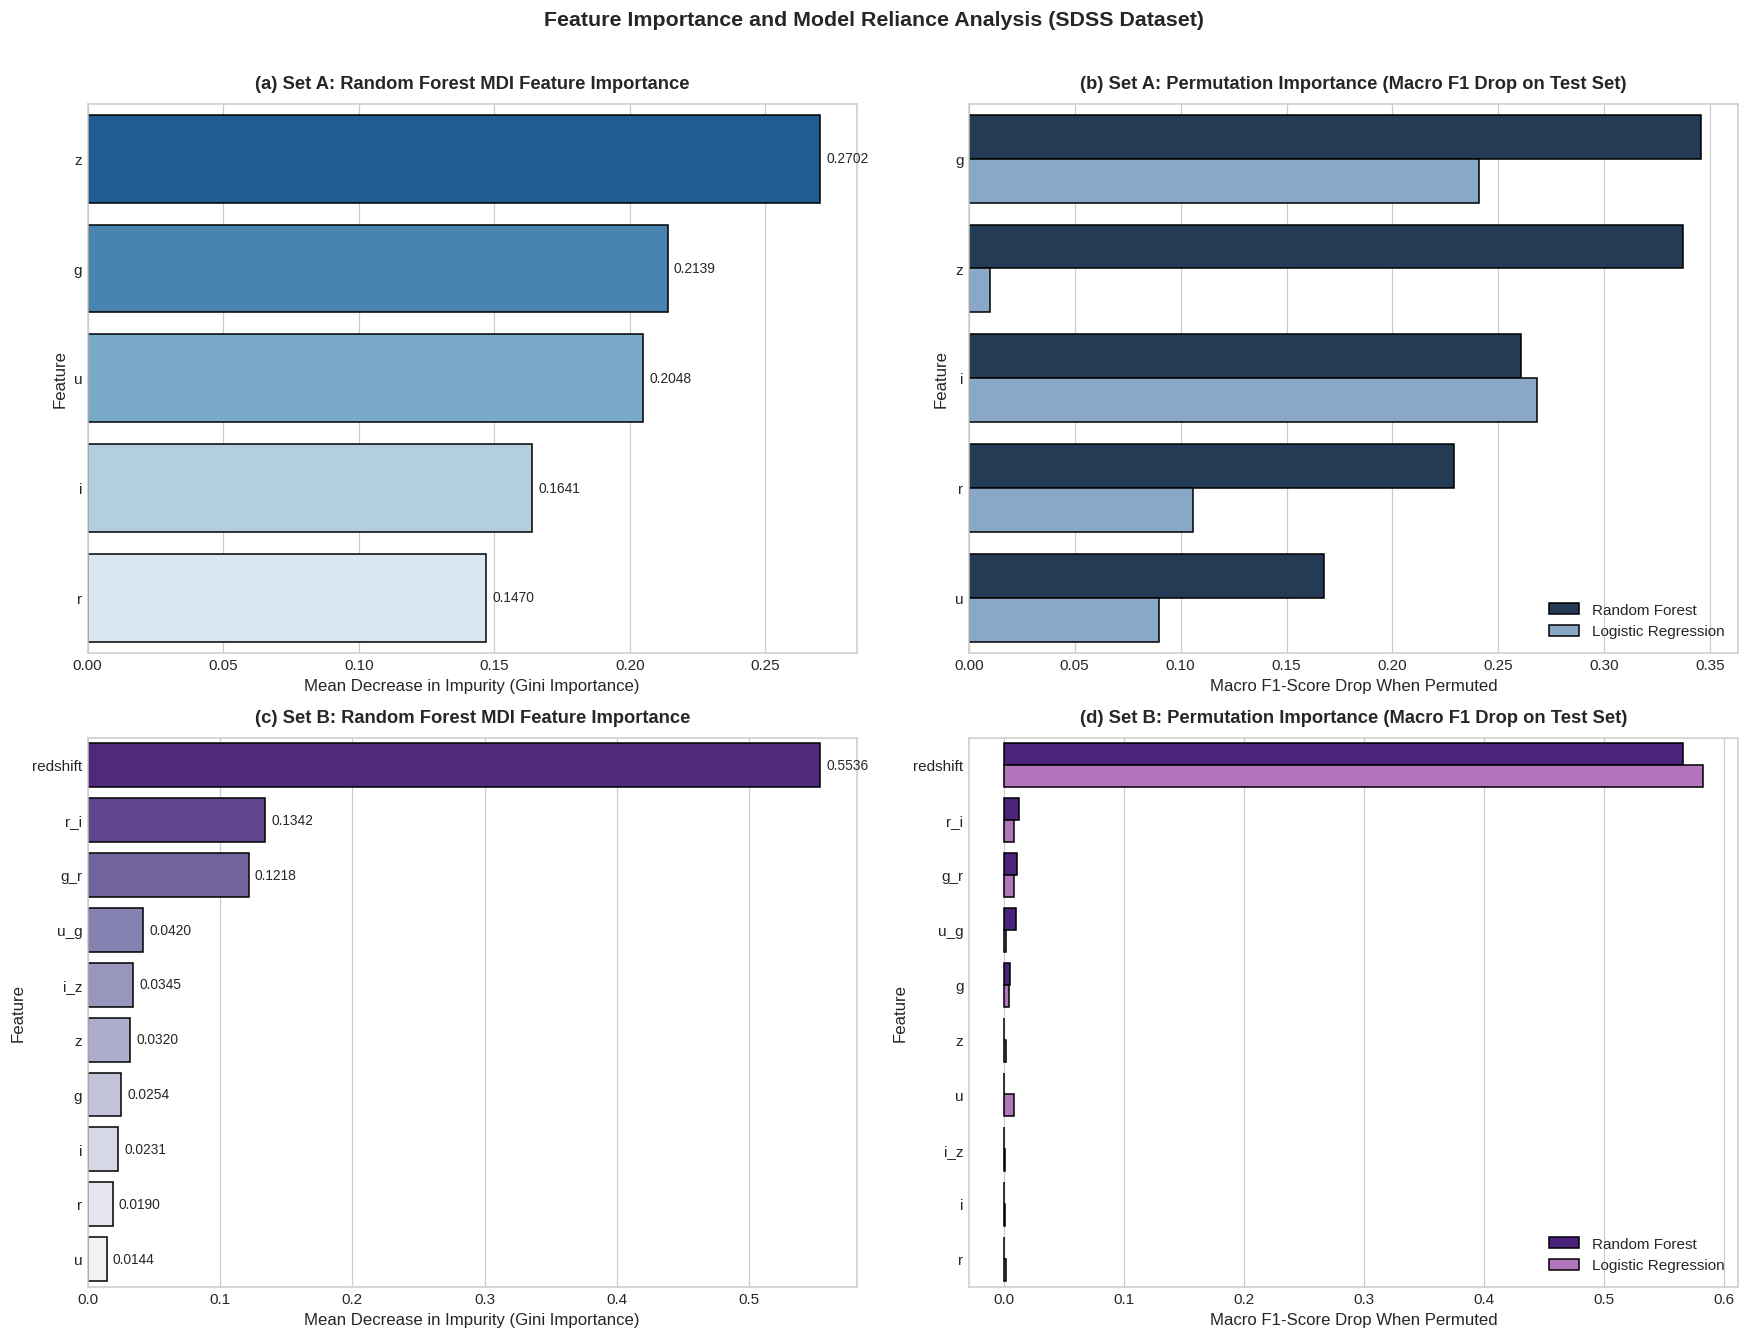
\includegraphics[width=0.72\textwidth]{figures/04_feature_importance_and_permutation_ranking.png}
    \caption{\textbf{Feature importance rankings.} In the 10-feature set, spectroscopic redshift accounts for over 55\% of tree impurity reduction, while optical colors ($r-i, g-r$) displace raw filter measurements.}
    \label{fig:04_importance_bars}
\end{figure}

Table~\ref{tab:04_importance_table} lists the rankings for the 10-feature expanded set.

\begin{table}[H]
\centering
\small
\caption{\textbf{Feature Importance Rankings in Feature Set B (Expanded Features)} on the held-out test set.}
\label{tab:04_importance_table}
\begin{tabular}{clcccc}
\toprule
\textbf{Rank} & \textbf{Feature} & \textbf{RF MDI Importance} & \textbf{Cumulative MDI} & \textbf{RF Permutation Drop} & \textbf{LR Permutation Drop} \\
\midrule
1 & \textbf{\texttt{redshift}} & \textbf{0.5536} & 0.5536 & \textbf{0.5661} & \textbf{0.5827} \\
2 & \textbf{\texttt{r\_i} (Color)} & \textbf{0.1342} & 0.6878 & 0.0123 & 0.0085 \\
3 & \textbf{\texttt{g\_r} (Color)} & \textbf{0.1218} & 0.8096 & 0.0112 & 0.0086 \\
4 & \textbf{\texttt{u\_g} (Color)} & 0.0420 & 0.8516 & 0.0098 & 0.0020 \\
5 & \textbf{\texttt{i\_z} (Color)} & 0.0345 & 0.8861 & 0.0002 & 0.0006 \\
6 & \textbf{$z$ (Infrared)} & 0.0320 & 0.9181 & 0.0004 & 0.0014 \\
7 & \textbf{$g$ (Green)} & 0.0254 & 0.9435 & 0.0048 & 0.0045 \\
8 & \textbf{$i$ (Near-IR)} & 0.0231 & 0.9666 & 0.0002 & 0.0012 \\
9 & \textbf{$r$ (Red)} & 0.0190 & 0.9856 & -0.0001 & 0.0020 \\
10 & \textbf{$u$ (UV)} & 0.0144 & 1.0000 & 0.0004 & 0.0082 \\
\bottomrule
\end{tabular}
\end{table}

\subsection{Progressive Subsets: The 3-Feature Miracle}
We evaluated models by adding features one by one ($k=1, 2, \dots$) in order of importance. Table~\ref{tab:04_subsets_b} and Figure~\ref{fig:04_subsets_combined} report the progression for Random Forest.

\begin{figure}[H]
    \centering
    \begin{subfigure}[b]{0.48\textwidth}
        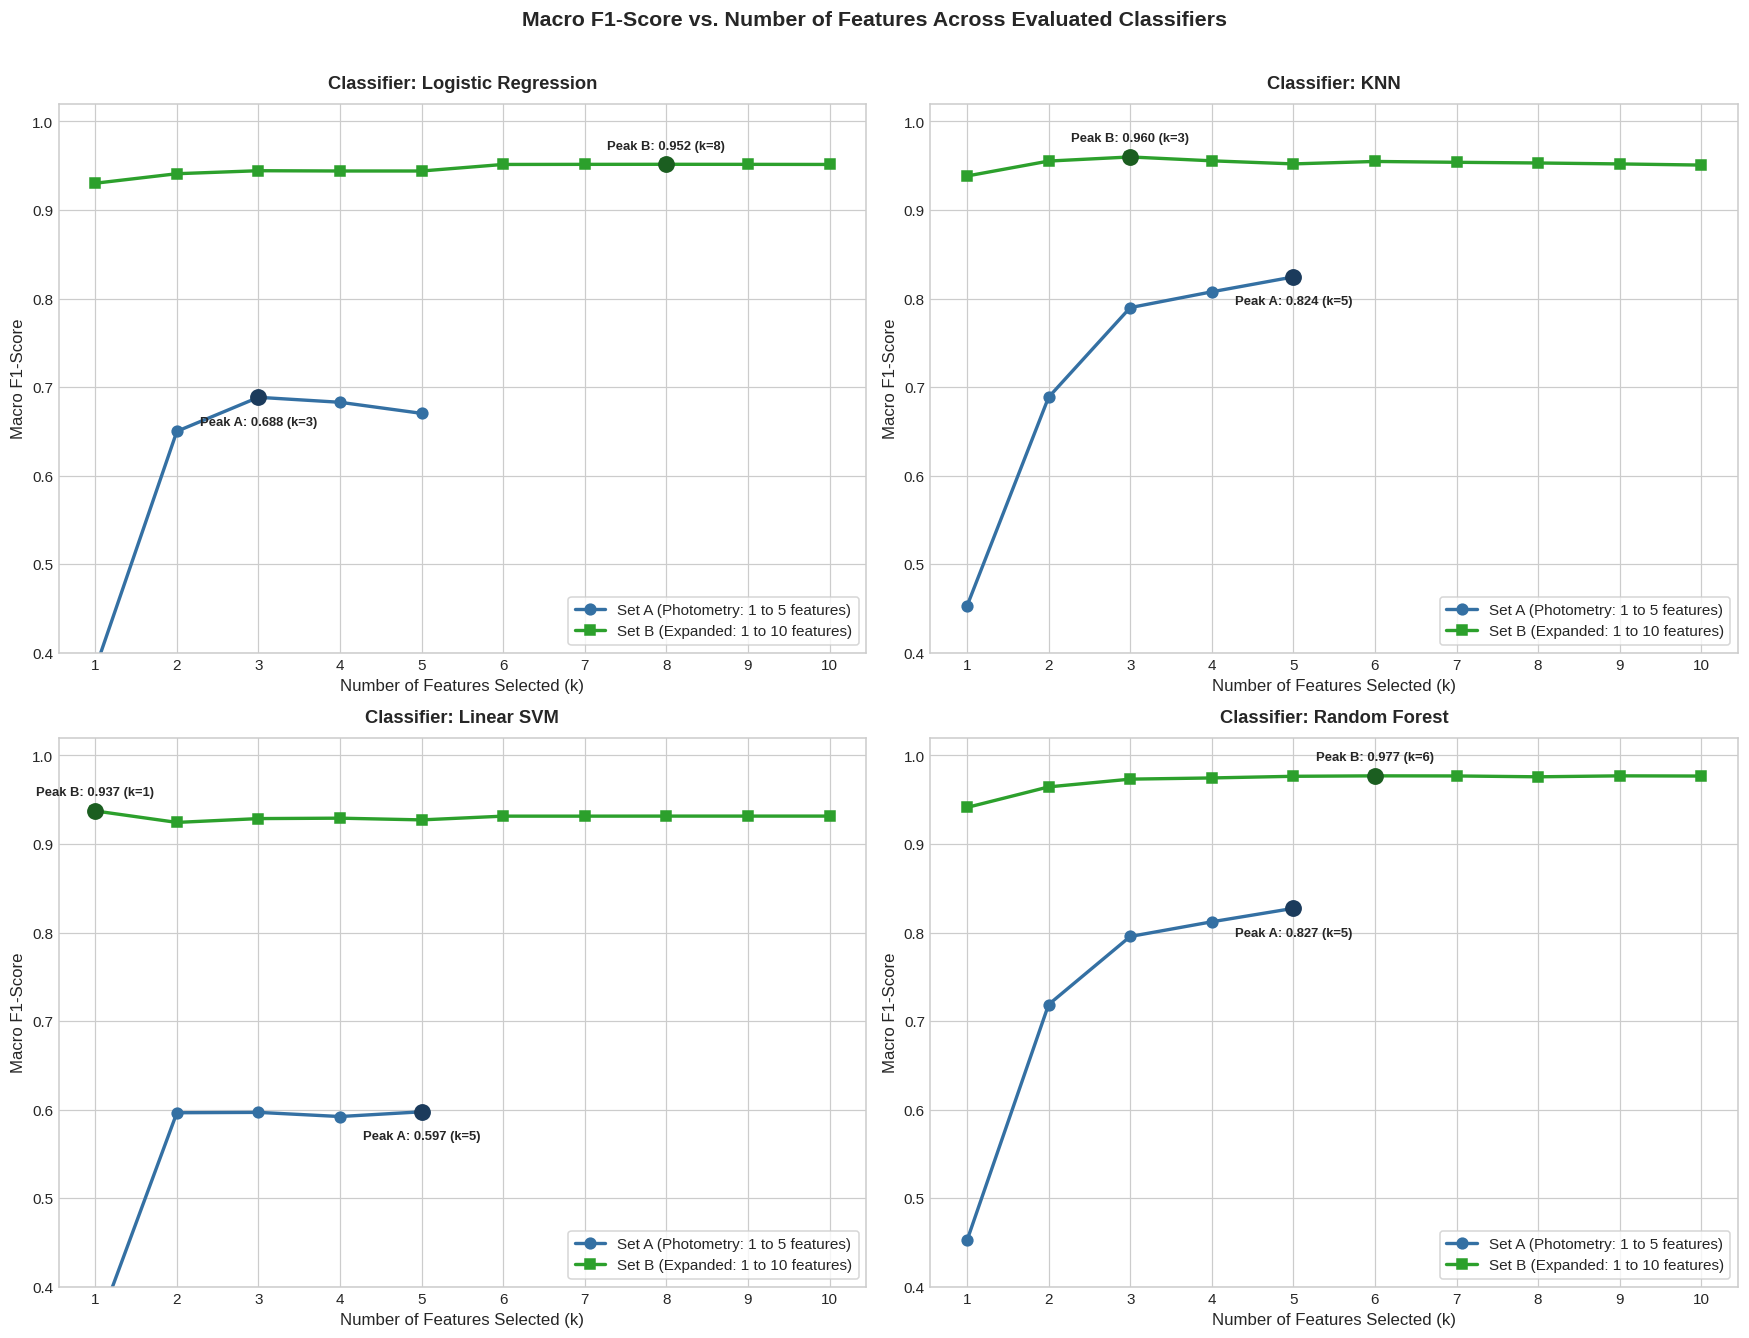
\includegraphics[width=\textwidth]{figures/04_macro_f1_vs_feature_count.png}
        \caption{Macro F1 vs. feature count ($k$).}
        \label{fig:04_k_vs_f1}
    \end{subfigure}
    \hfill
    \begin{subfigure}[b]{0.48\textwidth}
        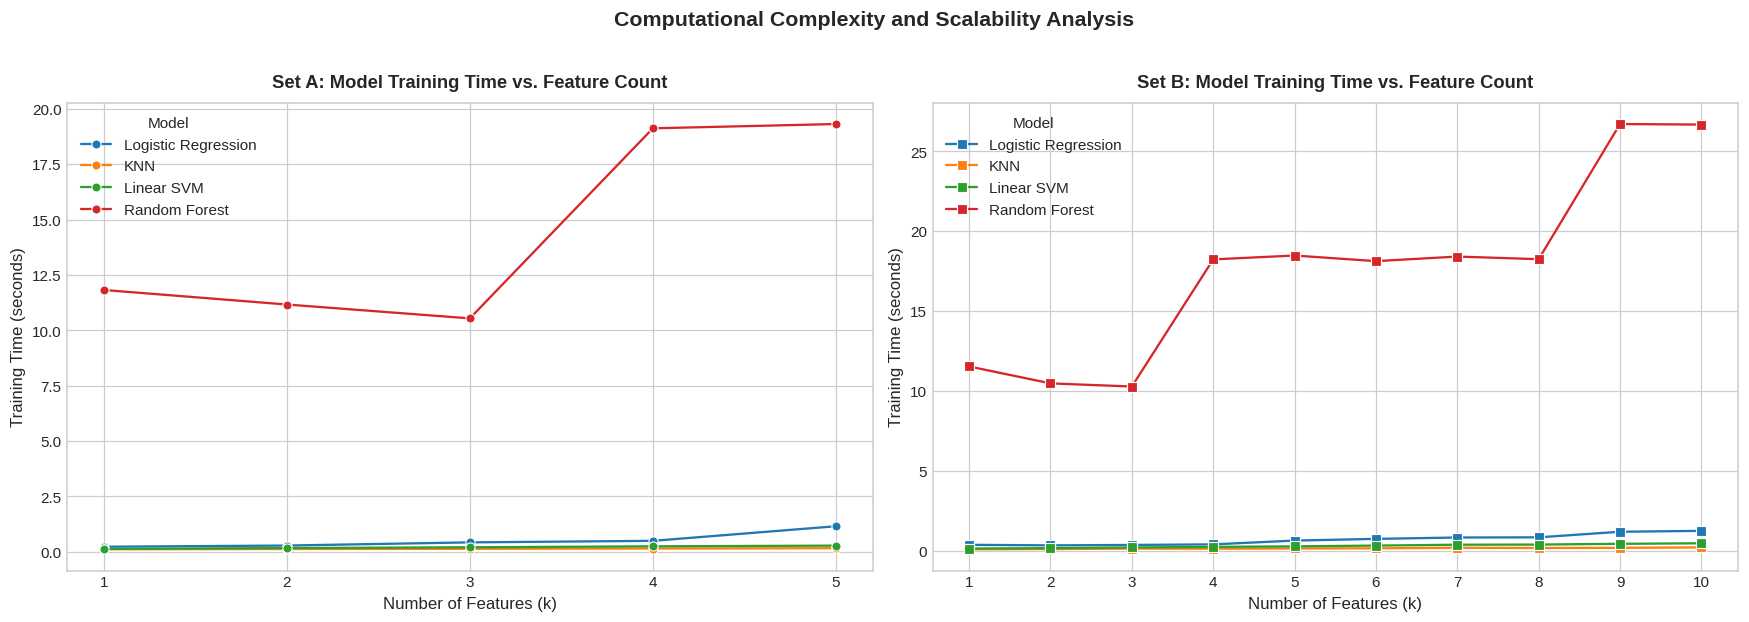
\includegraphics[width=\textwidth]{figures/04_training_time_vs_feature_count.png}
        \caption{Training time vs. feature count ($k$).}
        \label{fig:04_k_vs_time}
    \end{subfigure}
    \caption{\textbf{Progressive subset evaluation.} (a) Performance hits a plateau at $k=3$. (b) Training time jumps significantly beyond $k=3$ with no accuracy gain.}
    \label{fig:04_subsets_combined}
\end{figure}

\begin{table}[H]
\centering
\small
\caption{\textbf{Progressive Subset Results for Random Forest} in Feature Set B.}
\label{tab:04_subsets_b}
\begin{tabular}{clcccc}
\toprule
$k$ & \textbf{Features Included} & \textbf{Accuracy (\%)} & \textbf{Macro F1} & \textbf{Train Time (s)} & \textbf{Status} \\
\midrule
1 & \texttt{redshift} & 95.20\% & 0.9413 & 11.55 & High baseline \\
2 & \texttt{redshift}, $r-i$ & 96.95\% & 0.9645 & 10.49 & Very competitive \\
\textbf{3} & \textbf{\texttt{redshift}, $r-i, g-r$} & \textbf{97.71\%} & \textbf{0.9733} & \textbf{10.29} & \textbf{Smallest Competitive Subset} \\
4 & + $u-g$ & 97.82\% & 0.9746 & 18.25 & Marginal gain \\
5 & + $i-z$ & 97.98\% & 0.9765 & 18.49 & Marginal gain \\
\textbf{6} & \textbf{+ $z$ (Peak Subset)} & \textbf{98.03\%} & \textbf{0.9770} & \textbf{18.14} & \textbf{Maximum Score} \\
10 & Full 10-feature set & 98.01\% & 0.9768 & 26.68 & 2.6x slower than $k=3$ \\
\bottomrule
\end{tabular}
\end{table}

\textbf{Key Takeaways:}
\begin{itemize}[noitemsep]
    \item \textbf{In Feature Set B (Expanded):} A minimal \textbf{3-feature model (\texttt{redshift}, $r-i$, $g-r$)} achieves \textbf{0.9733 Macro F1} and \textbf{97.71\% Accuracy}. This captures \textbf{99.6\% of peak performance} while cutting training time from 18.14s down to 10.29s (a \textbf{43.2\% time savings}) and halving feature storage.
    \item \textbf{In Feature Set A (Photometry only):} A \textbf{3-feature model ($z, g, u$)} achieves \textbf{0.7955 Macro F1}, capturing \textbf{96.2\% of the 5-band baseline performance}.
\end{itemize}

% =========================================================================
% SECTION 6: PHASE 5 - UNCERTAINTY ANALYSIS
% =========================================================================
\section{Phase 5: Prediction Uncertainty and Error Analysis}

\subsection{The Core Idea: Moving Beyond Hard Guesses}
A model that makes predictions with 99.9\% confidence is very different from a model guessing with 35\% confidence. In this phase, we ask: \emph{Are predicted probabilities calibrated to reality? Can we use confidence scores to reject ambiguous objects and guarantee a pure catalog?}

\subsection{Confidence and Correctness}
We define prediction confidence as the highest probability assigned to any class:
\begin{equation}
    C = \max_{k} P(Y=k|x)
\end{equation}
Table~\ref{tab:05_confidence_tiers} and Figure~\ref{fig:05_conf_combined} show how accuracy changes across confidence tiers.

\begin{figure}[H]
    \centering
    \begin{subfigure}[b]{0.48\textwidth}
        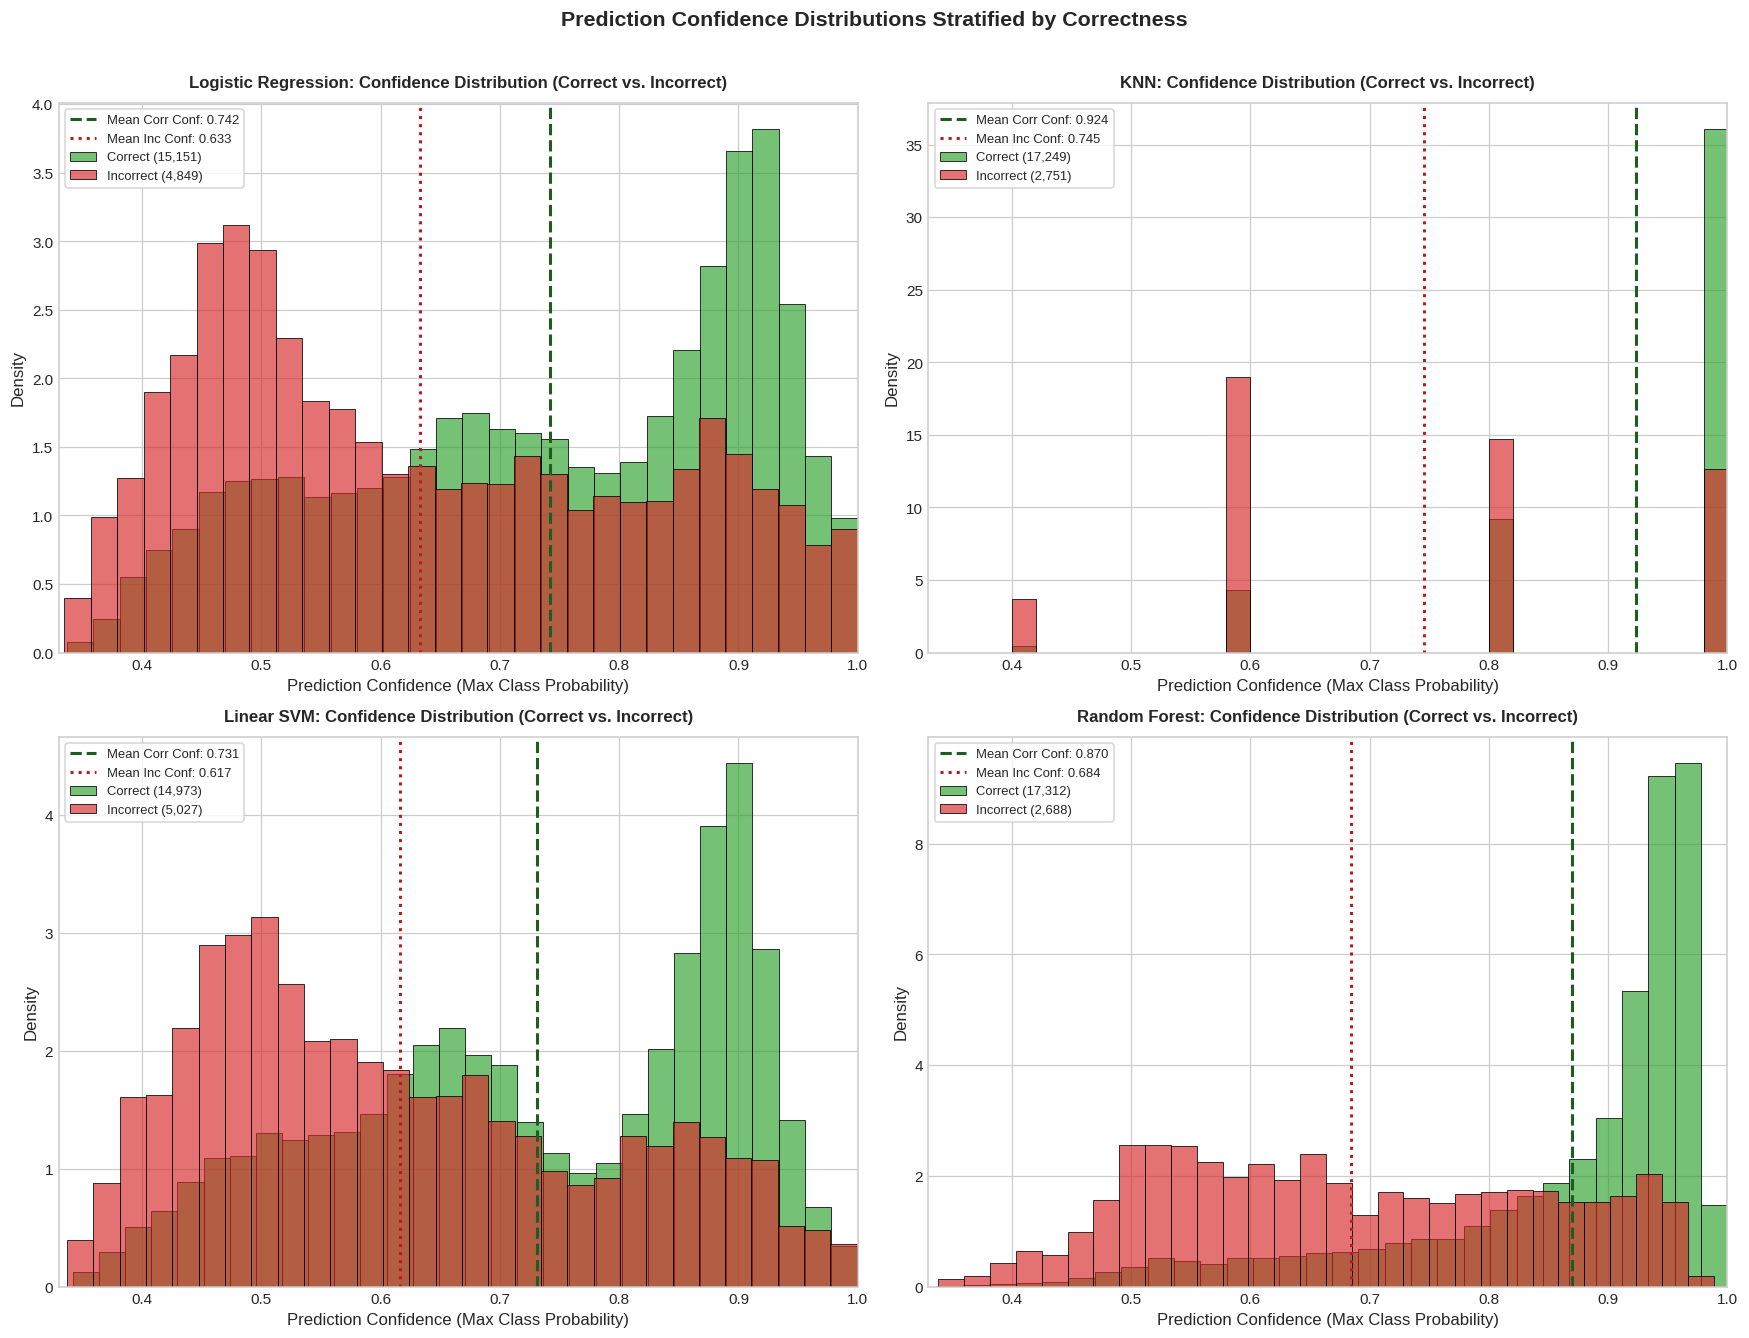
\includegraphics[width=\textwidth]{figures/05_confidence_distribution_by_correctness.png}
        \caption{Confidence of correct vs. wrong predictions.}
        \label{fig:05_conf_dist}
    \end{subfigure}
    \hfill
    \begin{subfigure}[b]{0.48\textwidth}
        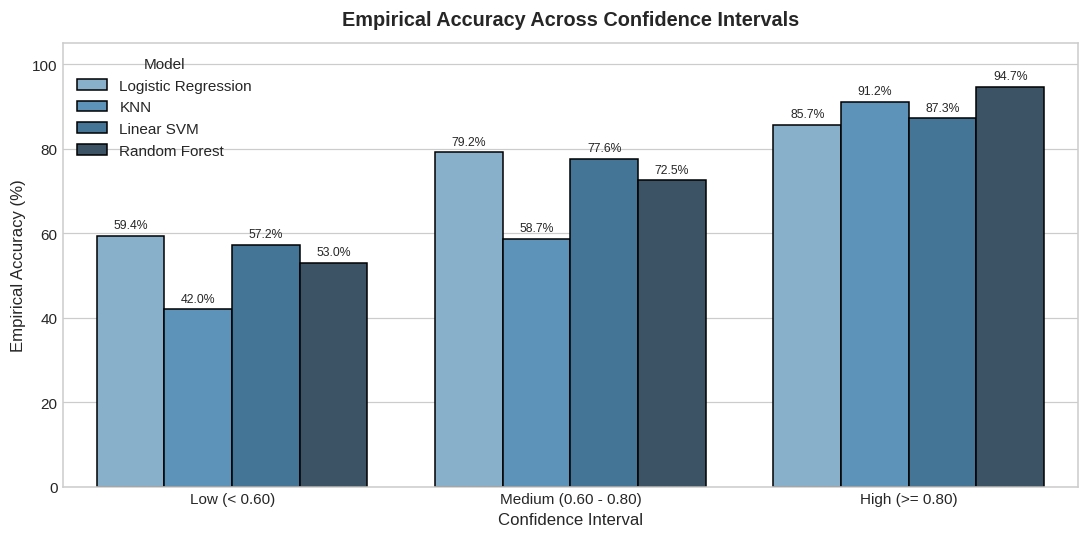
\includegraphics[width=\textwidth]{figures/05_accuracy_by_confidence_bins.png}
        \caption{Empirical accuracy across confidence tiers.}
        \label{fig:05_conf_bins}
    \end{subfigure}
    \caption{\textbf{Confidence analysis.} (a) Correct predictions (blue) cluster near 1.0; errors (red) shift toward lower confidence. (b) Accuracy rises steeply with higher confidence.}
    \label{fig:05_conf_combined}
\end{figure}

\begin{table}[H]
\centering
\small
\caption{\textbf{Accuracy across Confidence Tiers for Random Forest} on 20,000 test observations.}
\label{tab:05_confidence_tiers}
\begin{tabular}{lcccc}
\toprule
\textbf{Confidence Tier} & \textbf{Sample Count} & \textbf{Proportion (\%)} & \textbf{Empirical Accuracy} & \textbf{Error Rate} \\
\midrule
\textbf{Low ($< 0.60$)} & 2,056 & 10.28\% & \textbf{53.02\%} & \textbf{46.98\%} \\
\textbf{Medium ($0.60 - 0.80$)} & 3,477 & 17.39\% & \textbf{72.53\%} & 27.47\% \\
\textbf{High ($\ge 0.80$)} & 14,467 & \textbf{72.34\%} & \textbf{94.70\%} & \textbf{5.30\%} \\
\bottomrule
\end{tabular}
\end{table}

\textbf{Takeaway:} When Random Forest confidence is $\ge 0.80$ (which covers over 72\% of the data), accuracy is \textbf{94.70\%}. When confidence falls below 0.60, the model is practically guessing (53.02\% accuracy).

\subsection{Probability Calibration}
A model is well-calibrated if an 80\% probability means the model is right 80\% of the time. We measured Expected Calibration Error (ECE) across 10 bins (Figure~\ref{fig:05_calibration}).
\begin{itemize}[noitemsep]
    \item \textbf{Random Forest is remarkably calibrated:} It achieved an \textbf{ECE of 0.0222 (2.22\%)}. Its probabilities can be trusted directly as real statistical likelihoods.
    \item \textbf{Platt Scaling for SVM:} 5-fold cross-validated Platt scaling successfully converted raw SVM margins into calibrated probabilities with an ECE of 6.03\%.
\end{itemize}

\begin{figure}[H]
    \centering
    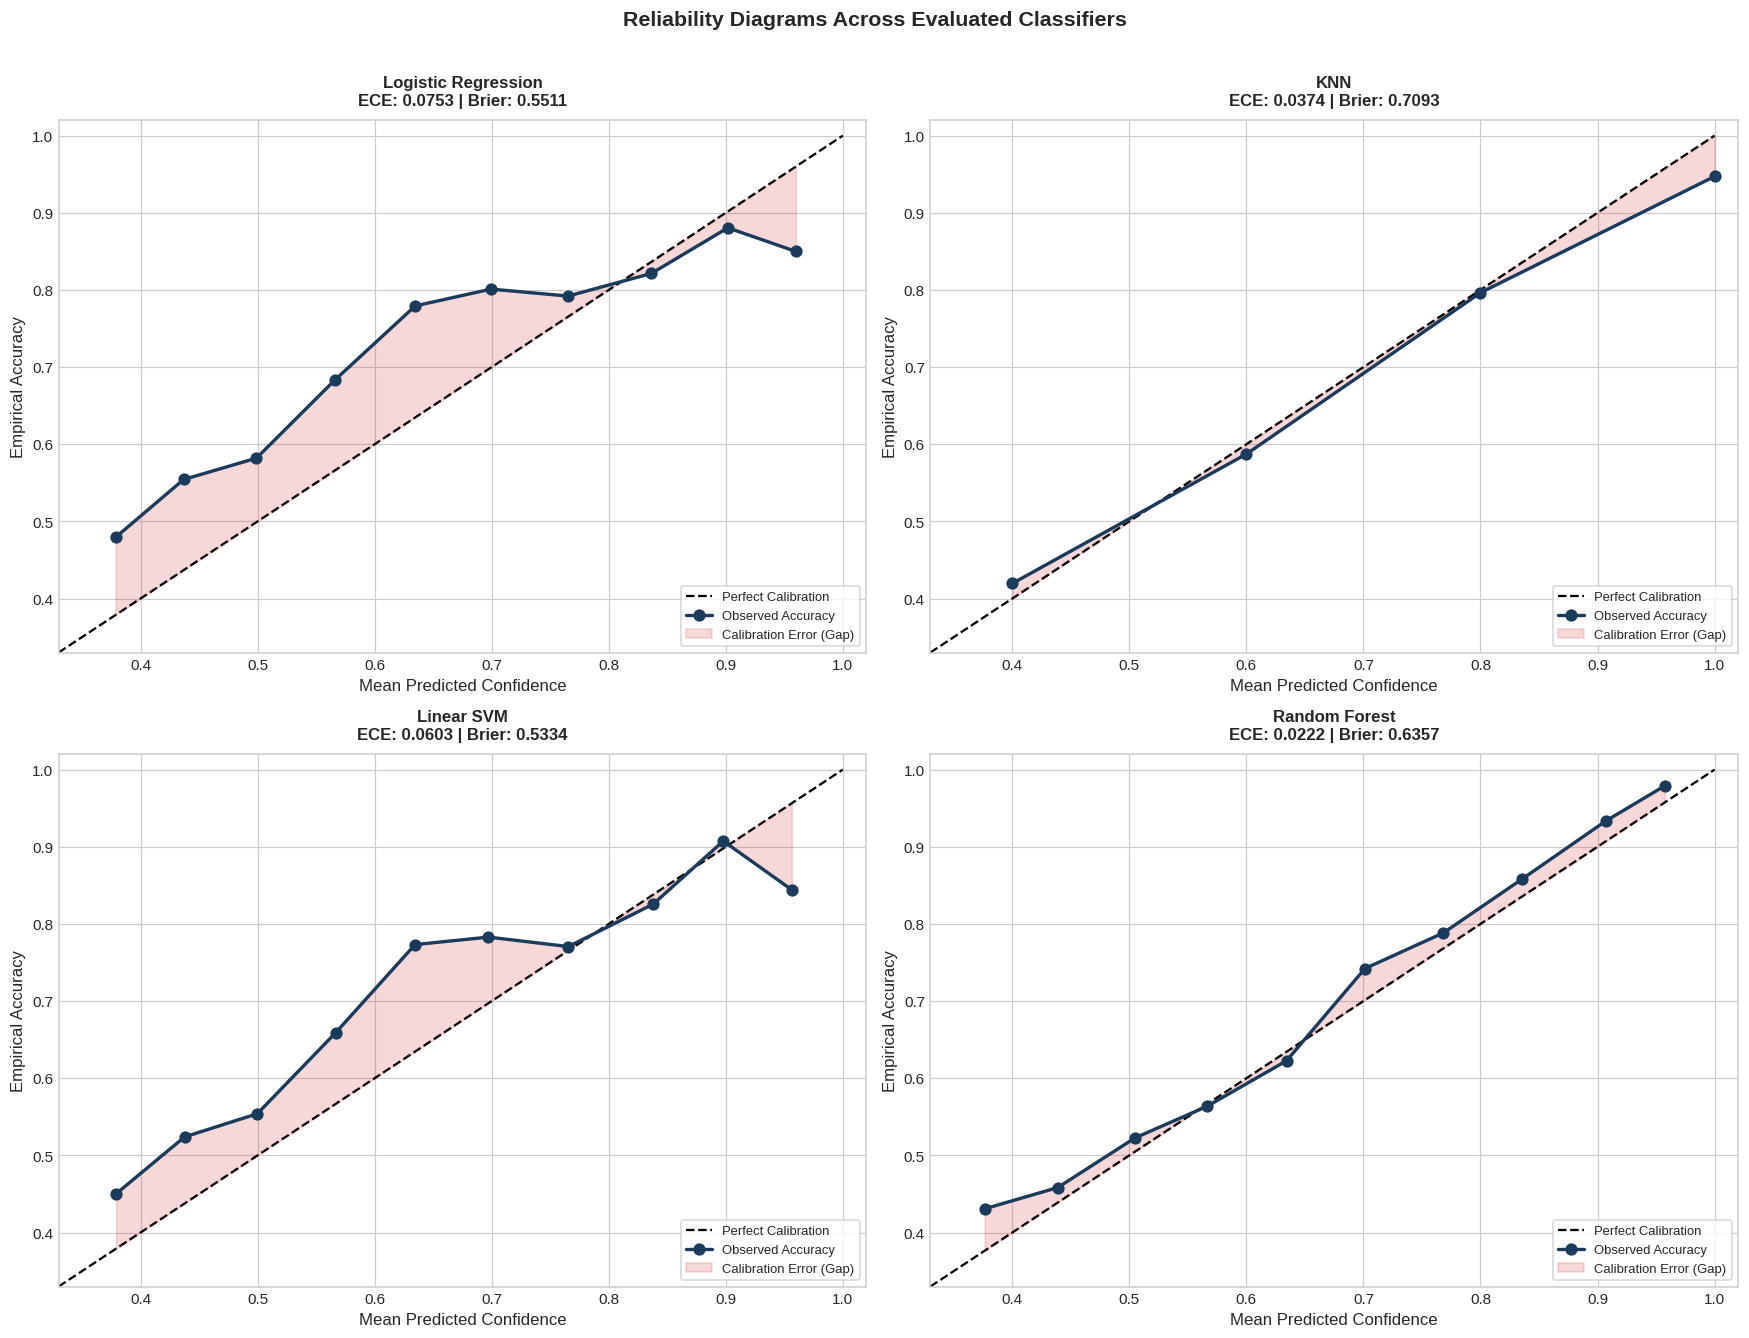
\includegraphics[width=0.62\textwidth]{figures/05_calibration_reliability_diagrams.png}
    \caption{\textbf{Reliability diagrams (calibration curves).} Random Forest (bottom-right) hugs the ideal diagonal line with an Expected Calibration Error of only 2.22\%.}
    \label{fig:05_calibration}
\end{figure}

\subsection{Model Consensus and Selective Prediction}
When all four models agree unanimously (77.47\% of test samples), collective accuracy is \textbf{90.20\%} (Table~\ref{tab:05_agreement}). On split decisions (14.23\% of samples), Random Forest and KNN are right \textbf{over 82\% of the time}, while linear models fail completely (~12\% accuracy).

\begin{table}[H]
\centering
\small
\caption{\textbf{Inter-Model Agreement Tiers} on 20,000 test samples.}
\label{tab:05_agreement}
\resizebox{\linewidth}{!}{
\begin{tabular}{lcccccc}
\toprule
\textbf{Consensus Tier} & \textbf{Count} & \textbf{Proportion (\%)} & \textbf{RF Acc} & \textbf{KNN Acc} & \textbf{LR Acc} & \textbf{SVM Acc} \\
\midrule
\textbf{Unanimous (4/4 Agree)} & 15,494 & \textbf{77.47\%} & \textbf{90.20\%} & 90.20\% & 90.20\% & 90.20\% \\
\textbf{Majority (3/4 Agree)}  & 1,660  & 8.30\%  & 58.13\% & 56.45\% & 48.73\% & 38.67\% \\
\textbf{Disagreement (Split)}  & 2,846  & 14.23\% & \textbf{83.31\%} & \textbf{82.08\%} & \textbf{12.86\%} & \textbf{12.47\%} \\
\bottomrule
\end{tabular}}
\end{table}

\begin{figure}[H]
    \centering
    \begin{subfigure}[b]{0.48\textwidth}
        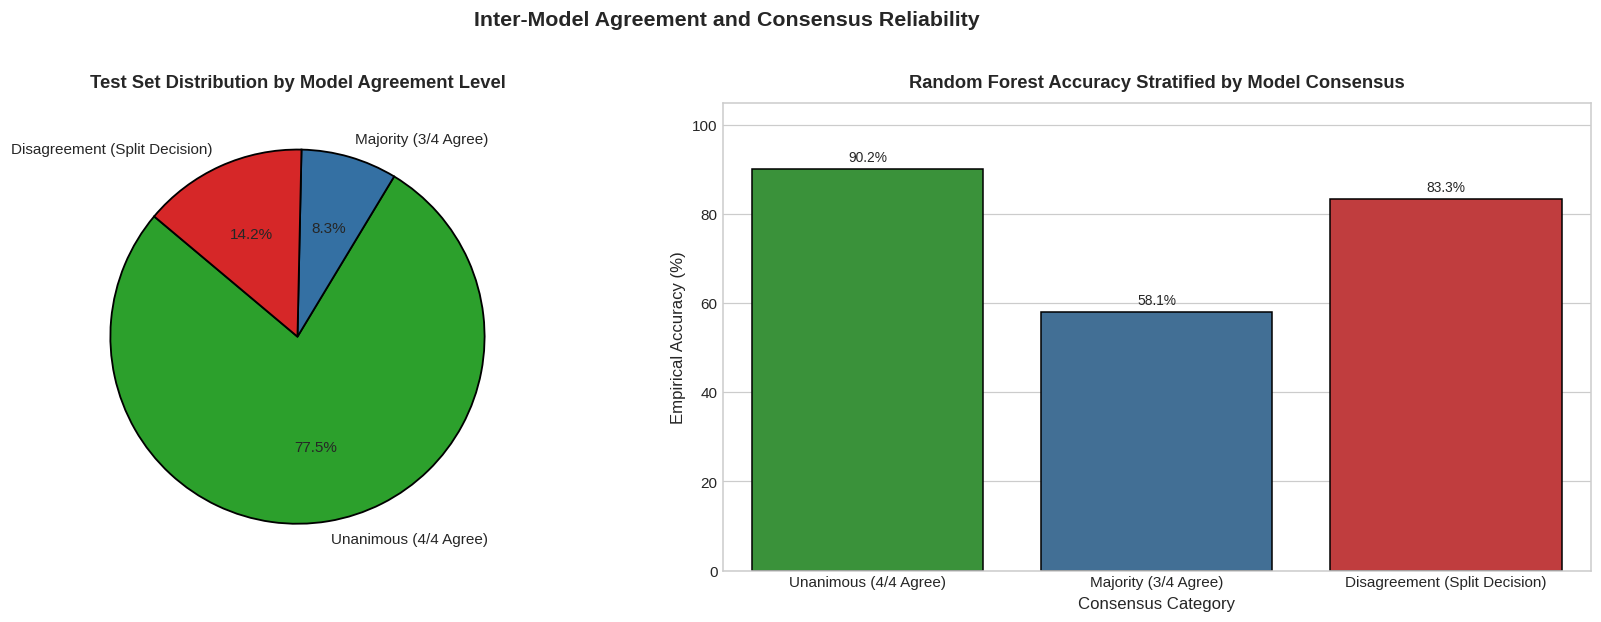
\includegraphics[width=\textwidth]{figures/05_model_agreement_and_consensus.png}
        \caption{Model accuracy by consensus level.}
        \label{fig:05_consensus}
    \end{subfigure}
    \hfill
    \begin{subfigure}[b]{0.48\textwidth}
        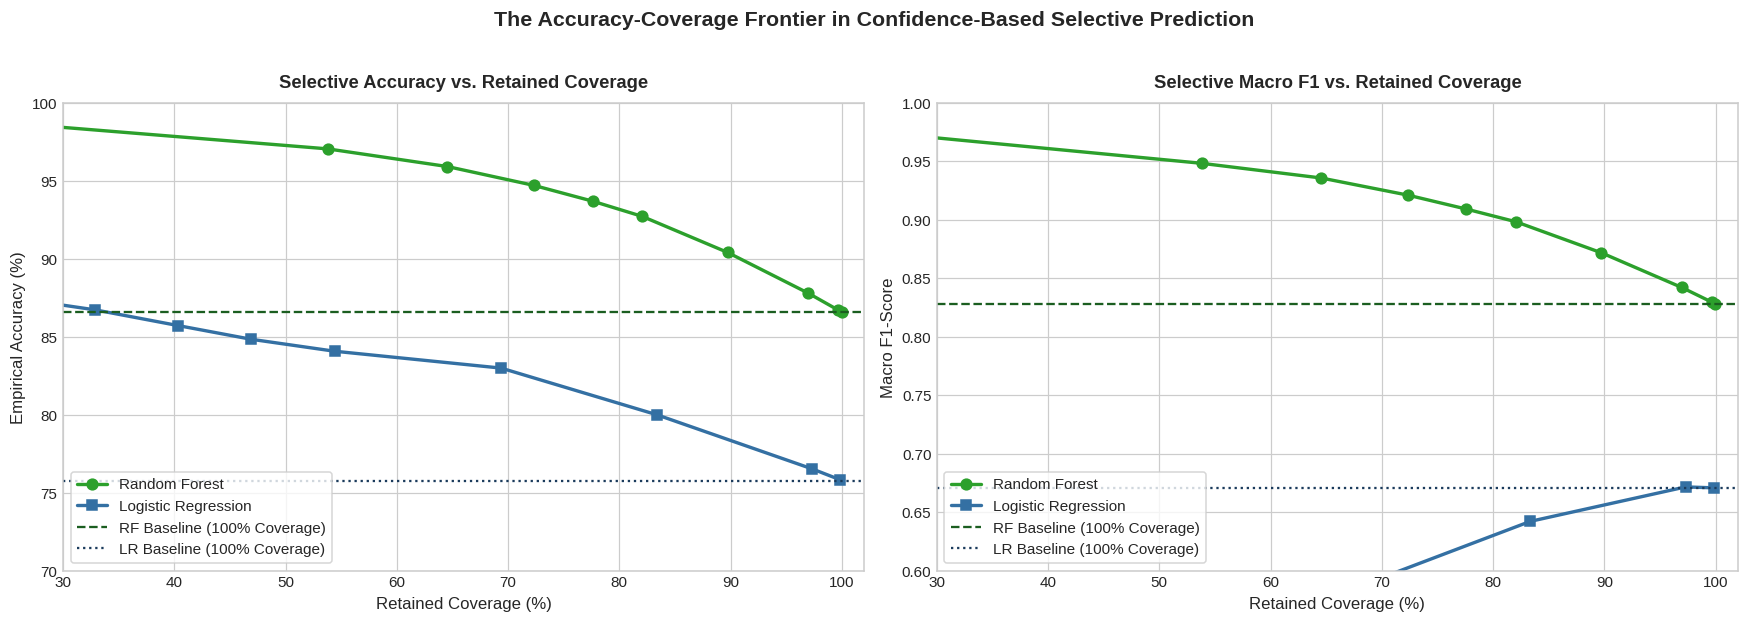
\includegraphics[width=\textwidth]{figures/05_selective_prediction_accuracy_coverage.png}
        \caption{Selective prediction frontier.}
        \label{fig:05_selective}
    \end{subfigure}
    \caption{\textbf{Consensus and selective prediction.} (a) In split decisions, non-linear models achieve >82\% accuracy while linear models collapse. (b) Tuning threshold $\tau$ trades survey coverage for pure accuracy.}
    \label{fig:05_agreement_combined}
\end{figure}

\textbf{Selective Prediction (Abstention):} By rejecting predictions below a threshold $\tau$, astronomers can trade coverage for purity (Table~\ref{tab:05_selective_results}):
\begin{itemize}[noitemsep]
    \item At $\tau = 0.80$, Random Forest achieves \textbf{94.70\% accuracy} on \textbf{72.34\% of the survey}.
    \item At $\tau = 0.95$, accuracy reaches \textbf{98.58\%} on \textbf{27.20\% of the survey}---matching the quality of an expensive spectroscopic survey using only camera images!
\end{itemize}

\begin{table}[H]
\centering
\small
\caption{\textbf{Selective Prediction Performance for Random Forest} across rejection thresholds.}
\label{tab:05_selective_results}
\begin{tabular}{ccccc}
\toprule
\textbf{Threshold ($\tau$)} & \textbf{Retained Samples} & \textbf{Retained Coverage (\%)} & \textbf{Retained Accuracy (\%)} & \textbf{Retained Macro F1} \\
\midrule
0.35 & 19,994 & 99.97\% & 86.58\% & 0.83 \\
0.60 & 17,944 & 89.72\% & 90.40\% & 0.87 \\
\textbf{0.80} & \textbf{14,467} & \textbf{72.34\%} & \textbf{94.70\%} & \textbf{0.92} \\
0.90 & 10,758 & 53.79\% & 97.04\% & 0.95 \\
\textbf{0.95} & \textbf{5,439} & \textbf{27.20\%} & \textbf{98.58\%} & \textbf{0.97} \\
\bottomrule
\end{tabular}
\end{table}

\begin{figure}[H]
    \centering
    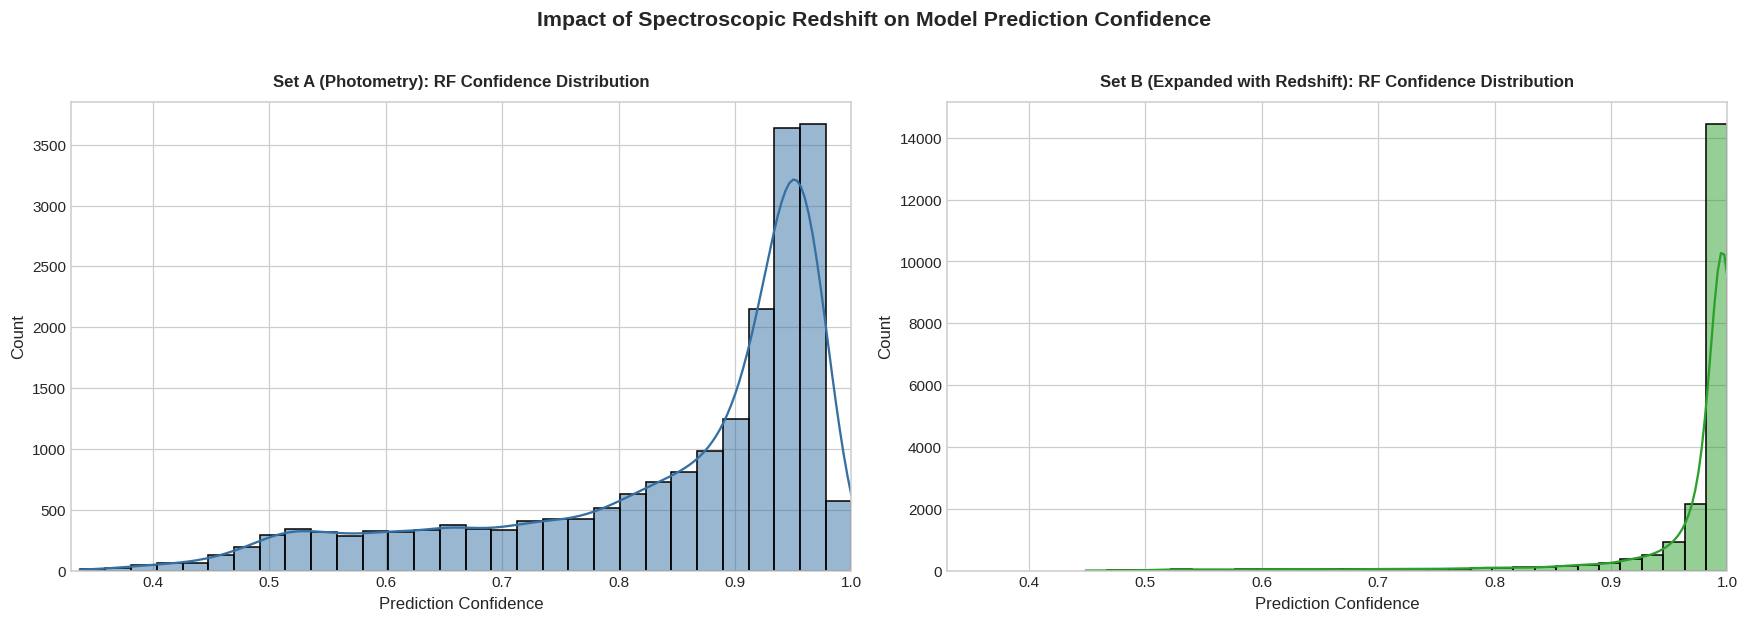
\includegraphics[width=0.62\textwidth]{figures/05_redshift_impact_on_confidence.png}
    \caption{\textbf{Confidence shift under expanded features.} When redshift is added (green), over 96.3\% of predictions surge into the ultra-high confidence tier ($\ge 0.80$).}
    \label{fig:05_redshift_conf}
\end{figure}

% =========================================================================
% SECTION 7: OVERALL SYNTHESIS & CONCLUSION
% =========================================================================
\section{Overall Synthesis and Practical Guidelines}

\subsection{The Complete Project Trajectory}
Table~\ref{tab:06_summary_trajectory} summarizes the entire arc of this semester project across all five experiments.

\begin{table}[H]
\centering
\small
\caption{\textbf{Complete Project Performance Trajectory} across the five experimental phases.}
\label{tab:06_summary_trajectory}
\resizebox{\linewidth}{!}{
\begin{tabular}{llccccl}
\toprule
\textbf{Phase} & \textbf{Experiment Focus} & \textbf{Features} & \textbf{Top Model} & \textbf{Accuracy} & \textbf{Macro F1} & \textbf{Key Discovery} \\
\midrule
\textbf{Phase 1} & Baseline Photometry & 5 & Random Forest & 86.56\% & 0.8277 & Linear models fail on stars (13.8\% recall). \\
\textbf{Phase 2} & Color Engineering & 9 & Random Forest & 88.47\% & 0.8514 & Colors boost Star F1 (+5.05 pp); 382 fewer errors. \\
\textbf{Phase 3} & Redshift Ablation & 10 & Random Forest & \textbf{98.00\%} & \textbf{0.9767} & Errors drop 85.2\% ($2,688 \to 399$); Linear models rescued. \\
\textbf{Phase 4} & Feature Selection & \textbf{3} & Random Forest & 97.71\% & 0.9733 & 3 features (\texttt{redshift}, $r-i, g-r$) retain 99.6\% of peak score. \\
\textbf{Phase 5} & Uncertainty \& Rejection & 5 & Random Forest & \textbf{94.70\%} & \textbf{0.9200} & Pure photometry reaches 94.7\% accuracy at 72.3\% coverage. \\
\bottomrule
\end{tabular}}
\end{table}

\subsection{Practical Rules for Astronomical Pipelines}
\begin{enumerate}[noitemsep]
    \item \textbf{For Real-Time Photometric Sky Surveys (No Redshift Available):}  
    Do not use raw magnitudes alone. Engineer color indices ($u-g, g-r, r-i, i-z$) and deploy Random Forest models. Implement confidence-based rejection at $\tau = 0.80$ to ingest 72\% of observations automatically with 94.7\% accuracy, sending the remaining 28\% to queue-based follow-up.
    \item \textbf{For Spectroscopic Surveys (Redshift Available):}  
    Do not build bulky 10-feature models. A compact 3-feature model using \texttt{redshift}, $r-i$, and $g-r$ provides 97.7\% accuracy with 43\% faster training and negligible storage.
    \item \textbf{Avoid Linear Models on Raw Magnitudes:}  
    Linear classifiers should never be deployed on raw apparent magnitudes without non-linear kernels, as they systematically mislabel stars as galaxies.
\end{enumerate}

\subsection{Conclusion}
This project demonstrates that automated pattern recognition can reliably classify astronomical objects. By engineering physical colors, isolating the value of redshift, reducing feature count, and measuring model confidence, we provide an accurate, fast, and transparent pipeline for modern survey astrophysics.

\end{document}
